% =====================================================================
%  Federated Retrieval-Augmentation:
%  Search as Individuation, Answers as Societies of Agents,
%  and Why a True Answer Can Be a Useless One
%
%  Self-contained. Every object is a finite weighted graph, a bounded
%  convex program, or a construction on one. All primitives are derived
%  from stated axioms; only standard, externally published literature is
%  cited. No companion manuscript is presupposed.
% =====================================================================
\documentclass[11pt,twocolumn,a4paper]{article}

\usepackage[utf8]{inputenc}
\usepackage[T1]{fontenc}
\usepackage{lmodern}
\usepackage[a4paper,margin=2.2cm,columnsep=0.55cm]{geometry}
\usepackage{amsmath,amssymb,amsthm,mathtools}
\usepackage{bm}
\usepackage{mathrsfs}
\usepackage{booktabs}
\usepackage{array}
\usepackage{enumitem}
\usepackage{microtype}
\usepackage{xcolor}
\usepackage{graphicx}
\usepackage{algorithm}
\usepackage{algpseudocode}
\usepackage[round,sort&compress]{natbib}
\usepackage[colorlinks=true,linkcolor=blue!45!black,
            citecolor=blue!45!black,urlcolor=blue!45!black]{hyperref}
\usepackage{cleveref}

% ---- theorem environments ----
\newtheoremstyle{frathm}{\topsep}{\topsep}{\itshape}{}{\bfseries}{.}{.5em}{}
\theoremstyle{frathm}
\newtheorem{theorem}{Theorem}[section]
\newtheorem{lemma}[theorem]{Lemma}
\newtheorem{proposition}[theorem]{Proposition}
\newtheorem{corollary}[theorem]{Corollary}
\theoremstyle{definition}
\newtheorem{definition}[theorem]{Definition}
\newtheorem{axiom}{Axiom}
\newtheorem{construction}[theorem]{Construction}
\newtheorem{example}[theorem]{Example}
\newtheorem{principle}[theorem]{Principle}
\newtheorem{binv}[theorem]{Invariant}
\theoremstyle{remark}
\newtheorem{remark}[theorem]{Remark}
\newtheorem{notation}[theorem]{Notation}

\crefname{axiom}{Axiom}{Axioms}
\Crefname{axiom}{Axiom}{Axioms}
\crefname{binv}{Invariant}{Invariants}
\Crefname{binv}{Invariant}{Invariants}

% ---- notation ----
\newcommand{\R}{\mathbb{R}}
\newcommand{\N}{\mathbb{N}}
\newcommand{\Gph}{\Gamma}
\newcommand{\V}{V}
\newcommand{\E}{E}
\newcommand{\wt}{w}
\newcommand{\med}{\mathsf{m}}
\newcommand{\flo}{\beta}
\newcommand{\cut}{\partial}
\newcommand{\co}{\complement}
\newcommand{\str}{\sigma}
\newcommand{\res}{\rho}
\newcommand{\rec}{M}
\newcommand{\Tab}{\mathcal{T}}
\newcommand{\Proc}{\Pi}
\newcommand{\Walk}{W}
\newcommand{\Om}{\Omega}
\newcommand{\al}{a}
\newcommand{\dem}{D}
\newcommand{\colA}{A}
\newcommand{\colB}{B}
\newcommand{\Char}{\chi}
\newcommand{\Rec}{\mathcal{R}}
\newcommand{\Know}{\mathcal{K}}
\newcommand{\Cands}{\mathcal{X}}
\newcommand{\Verd}{\mathsf{V}}
\newcommand{\Scene}{\mathsf{S}}
\newcommand{\scenes}{\mathcal{S}}
\newcommand{\price}{p^{\star}}
\newcommand{\drive}{\Phi}
\newcommand{\Purp}{x^{\star}}
\newcommand{\Ord}{R}
\newcommand{\phase}{\phi}
\newcommand{\Soc}{\Sigma}
\newcommand{\Out}{\mathcal{O}}
\newcommand{\Cell}{\mathrm{cell}}
\newcommand{\pot}{\kappa}
\newcommand{\Fed}{\mathsf{F}}
\newcommand{\Self}{\Gamma}
\newcommand{\alloc}{\mathbf{a}}
\newcommand{\att}{\alpha}
\newcommand{\abs}[1]{\lvert#1\rvert}
\newcommand{\norm}[1]{\lVert#1\rVert}
\newcommand{\eps}{\varepsilon}
\DeclareMathOperator{\Aut}{Aut}
\DeclareMathOperator*{\argmax}{arg\,max}
\DeclareMathOperator*{\argmin}{arg\,min}

\title{\textbf{Federated Retrieval-Augmentation:\\[3pt]
Search as Individuation, Answers as Societies of Agents,\\
and Why a True Answer Can Be a Useless One}}

\author{%
Kundai Farai Sachikonye\\
\small AIMe Registry for Artificial Intelligence\\
\small \texttt{kundai.sachikonye@bitspark.com}}

\date{\today}

\begin{document}
\maketitle

% =====================================================================
\begin{abstract}
\noindent
A retrieval-augmented system that returns a passage whose tokens match
the query, drawn from a source that is true, can still be useless to the
person who asked. We give a formal account of why this failure is not a
ranking defect to be tuned away but a category error forced by treating
\emph{content} as though it were \emph{meaning}. We develop the account
entirely in finite weighted graphs. A corpus, a knowledge base, and a
querying agent are each a \emph{contact graph}: a finite weighted graph
with a distinguished vertex, the \emph{medium}, standing for everything
not yet individuated. From the single hypothesis that the medium is never
exhausted by any finite retrieval process, we derive a strictly positive
\emph{resolution floor} on every result: no retrieval returns a point, only
a bounded region, and \emph{content}---a passage's literal tokens---and
\emph{meaning}---the passage's individuating cut against a specific
querying agent's own graph---provably come apart. We prove a
\textbf{recognition/search identity}: retrieving for a query and
recognising a match are inverse readings of one relation, so there is no
third, privileged place, neither in the corpus nor in the querier, where
"the answer" resides; it exists only as the joint fact of a decode. We
prove \textbf{receiver-relativity}: the same passage registers a different,
equally correct cell in different querying agents, so a single global
relevance score is not merely imprecise but is asking a question that has
no receiver-independent answer. We then replace the retrieve-then-generate
pipeline with a \textbf{society of split-attention agents}: each pipeline
stage is a bounded agent with its own conserved identity, its own purpose
as the attractor of a strongly convex drive, and a finite attention budget
it divides by a provably optimal water-filling rule across concurrently
competing information sources (\emph{scenes}). Retrieval becomes
\textbf{individuation, not lookup}: the causal propagation table
$\Tab(v_0,x^{\star},\Proc)$, evaluated at a trivial process, returns a
static knowledge-graph catalogue; evaluated at a nontrivial process, it
returns a generated answer; the two are one object at two settings of one
argument. Coherence of a returned claim requires a strongly connected
cycle of \emph{at least three} independently sourced, mutually supporting
retrieval catalysts, never a single passage and never two; and a search
terminates by \textbf{closure}---no further available source can add a new
answer class---never by a confidence threshold crossing, with contested
closure (irreconcilable sources) reported as a first-class output rather
than silently resolved by picking one. Cross-checking answers drawn from
sources with no shared internal representation (a trained domain adapter
against a symbolic index, or two independently fine-tuned models) is
certified by a \textbf{four-column relaxation} to \emph{semantic
quiescence}, which audits the \emph{route}---what each answer would
provoke as a follow-up---rather than the surface content, catching the
false-friend failure in which two sources agree lexically while diverging
in what they individuate. We instantiate the architecture as a concrete
revision of the Four-Sided Triangle pipeline for a bounded research-group
deployment: internal documents, domain-adapted models, and structured
records are federated receivers in one contact graph, queried by
individuation against a specific researcher's own decoder rather than
scored against a receiver-independent notion of relevance. We report a
validation suite of reproducible, seeded computational experiments against
every load-bearing claim, stored as machine-readable JSON records.
\end{abstract}

\noindent\textbf{Keywords:} retrieval-augmented generation; individuation
by negation; resolution floor; content versus meaning; receiver-relativity;
causal propagation table; water-filling attention allocation; coherence
triangle; closure; four-column relaxation; federated search; split-attention
agents.

\tableofcontents

% =====================================================================
\part{Foundations: Why a True Result Can Be a Useless One}
% =====================================================================

% =====================================================================
\section{Introduction}
\label{sec:intro}
% =====================================================================

\subsection{The failure this paper explains}

Consider the ordinary operation of a retrieval-augmented generation
system built the standard way: a query is embedded, the embedding is
compared against a vector index of chunked documents, the top-$k$ chunks
by cosine similarity are retrieved, and a language model is asked to
answer using them. The system returns a passage. The passage is drawn
from a genuine, peer-reviewed, factually accurate source. Its tokens
substantially overlap the query's tokens, which is why the retriever
ranked it first. And it does not answer the question the researcher
asked, because the researcher's question was never really about those
tokens; it was about a specific configuration of a specific problem in a
specific project, for which the retrieved passage is a true statement
about something adjacent, not a statement about that.

This is not a tuning failure correctable by a better embedding model, a
reranker, or a larger retrieved-context window. We will argue, and prove
in the formal development below, that it is the symptom of a category
error: the retrieval step optimises \emph{content fidelity}---how well the
returned string's literal tokens match the query's---while what the
researcher requires is \emph{meaning fidelity}---whether the returned
material individuates the same thing the researcher is individuating,
relative to what that researcher already holds fixed. These are, in
general, different targets, and a system tuned against the first can
degrade arbitrarily against the second while its reported relevance
scores improve. A true, well-sourced, high-similarity passage is exactly
the object this paper explains as \emph{useless}: correct content,
mismatched meaning.

\subsection{The library, restated formally}

An intuition motivates the formal development and is worth stating
before the machinery, though no theorem below depends on it. A search
engine and its user resemble a person standing before the shelves of a
library. Neither the books nor the person holds the answer prior to the
encounter: a book does not know, of itself, whether it is the answer to
a question that has not been asked of it, and a person does not know, in
advance of consulting the shelves, exactly which book will resolve their
question. The answer is not stored in either party; it is constituted by
the act of a specific person consulting a specific shelf under a specific
question, and a different person consulting the same shelf under the
same words may correctly arrive elsewhere. Two complementary strands of
a DNA molecule offer the same structural point in a different register:
neither strand, read alone, is the genetic information; the strands are
different \emph{representations} related by a fixed complementarity rule,
and the invariant that is transmitted is a property of the paired
structure, not of either sequence in isolation. We will show, as
theorems rather than as this analogy, that a retrieval result is
structurally the same kind of object: never a fact residing in a
document, never a fact residing in a query, but a joint individuation
computed against a medium that belongs to neither.

\subsection{What this paper contributes}

\begin{enumerate}[leftmargin=1.4em,itemsep=2pt]
\item \textbf{The resolution floor for retrieval} (\Cref{sec:floor}). We
derive, from the single hypothesis that the search medium is never
exhausted, a strictly positive floor $\flo>0$ on every retrieval: no
result is a point, every result is a bounded region.
\item \textbf{Content and meaning provably diverge}
(\Cref{sec:content-meaning}). We prove that a passage's content (its
literal tokens) and its meaning (its individuating cut against a specific
receiver's graph) coincide only in the degenerate case where the literal
form is itself the operative individuation, and exhibit the general case
in which a content-optimal retrieval is meaning-suboptimal by a
quantity bounded away from zero.
\item \textbf{The recognition/search identity and receiver-relativity}
(\Cref{sec:individuation}). We prove that querying and recognising a
match are inverse readings of one relation, so there is no
receiver-independent fact of relevance; distinct researchers correctly
register distinct cells for the same passage, at their own floor, with
no privileged registration among them.
\item \textbf{Retrieval as individuation via the causal propagation
table} (\Cref{sec:table}). We show a static knowledge index and a
generative retrieval-augmented answer are one table,
$\Tab(v_0,x^{\star},\Proc)$, evaluated at two settings of a process
argument, unifying "look it up" and "reason it out" as the same
operation.
\item \textbf{Coherence and closure as the correct stopping and grounding
rules} (\Cref{sec:catalysis}). We prove that a claim is robustly grounded
only by a strongly connected triangle of independent sources, never one
passage and never two, and that a search is correctly terminated by
\emph{closure}---no further available source adds a new answer class---which
we prove strictly stronger than any confidence threshold.
\item \textbf{The four-column route-audit for cross-source verification}
(\Cref{sec:relaxation}). We construct a relaxation that certifies
agreement between sources with no shared internal representation by
comparing what each source's answer \emph{provokes}, catching false
friends invisible to endpoint-only comparison.
\item \textbf{The society-of-agents architecture}
(\Cref{sec:architecture}). We replace the fixed sequential
retrieve-then-generate pipeline with a society of bounded, split-attention
agents, each a node of one contact graph, coordinating via a shared
outcome space rather than a shared representation, and dividing attention
across concurrently competing sources by a provably optimal water-filling
rule.
\item \textbf{A concrete instantiation for a bounded research-group
deployment} (\Cref{sec:deployment}). We specify how the architecture
federates internal documents, domain-adapted models, and structured
records as receivers in one contact graph queried by individuation
against a named researcher's own decoder.
\item \textbf{Validation} (\Cref{sec:validation}). We report a seeded,
reproducible computational suite checking every load-bearing theorem on
explicitly constructed instances, with results stored as JSON records.
\end{enumerate}

\subsection{Method}

Every object below is a finite weighted graph, a bounded map between
finite sets, or a construction on one. Minimum cuts are exact and
computable by maximum flow~\citep{fordfulkerson1956,menger1927}. We
introduce no probability measure and no metric beyond a derived
normalisation on $[0,1]$; where an uncertainty is required it is the
graph's own floor-distance, forced by the construction rather than
posited by a prior or a membership function. Words with an evocative
reading---``content,'' ``meaning,'' ``relevance,'' ``coherence''---each
name a specific graph-theoretic object defined in the text; no theorem
depends on any reading beyond that definition. Interpretive remarks are
marked as such and are never load-bearing.

% =====================================================================
\section{The Search Medium and Its Floor}
\label{sec:floor}
% =====================================================================

\subsection{Contact graphs for retrieval}

\begin{definition}[Contact graph; the medium]
\label{def:contact}
A \emph{contact graph} is a finite weighted graph $\Gph=(\V,\E,\wt)$,
$\wt:\E\to\R_{>0}$, together with a distinguished vertex $\med\in\V$, the
\emph{medium}, adjacent to every other vertex. Vertices $v\neq\med$ are
\emph{claims}: candidate individuated units of information---a document
chunk, a database record, a structured fact, a model-generated
statement. An edge $\{u,v\}$ is a \emph{contact}; its weight is the cost
of the distinction separating $u$ from $v$. The medium stands for
everything not yet individuated, without regard to whether it is stored
on a local index, a remote corpus, or the weights of a trained model.
\end{definition}

\begin{remark}[No boundary between local, remote, and learned]
\label{rem:no-boundary}
\Cref{def:contact} draws no distinction between a claim recoverable from
a locally indexed document, one recoverable from a remote database, and
one recoverable only by an inference from a trained model's parameters:
all three are, prior to individuation, contents of the single vertex
$\med$. This licenses the federation of \Cref{sec:architecture}: a
retrieval pipeline may draw candidate claims from a full-text index, a
knowledge graph, and a domain-adapted language model as computationally
uniform sources, because the graph encodes only a cost of separation, never
a storage medium.
\end{remark}

\begin{definition}[Separation cost]
\label{def:sepcost}
The \emph{separation cost} of a claim $v$ is
$\str(v)=\min_{S\ni v,\,\med\notin S}\wt(\cut(S))$, attained since $\V$ is
finite; the minimising cut is $v$'s \emph{resting cut}.
\end{definition}

\subsection{Non-completability and the floor theorem}

\begin{definition}[Non-completable medium]
\label{def:noncompletable}
An \emph{expanding retrieval family} is a chain of contact graphs
$\Gph_0\subseteq\Gph_1\subseteq\cdots$, each obtained from the last by
adding claims and contacts while retaining the medium and all prior
structure. The medium is \emph{non-completable} if the family has no
terminal stage: for every finite $\Gph_k$ there is $\Gph_{k+1}
\supsetneq\Gph_k$. This is an order condition---no last stage of
retrieval---not a claim about the cardinality of the corpus.
\end{definition}

\begin{remark}[Why a retrieval medium is non-completable]
\label{rem:why}
For any finite index---however large the corpus, however well the model
was trained---there is a further document not yet ingested, a further
record not yet linked, a further inference not yet drawn. This is the
formal content of the observation that a research group's internal
corpus, once federated with external literature and a trained model's own
generative capacity, has no boundary at which retrieval could in
principle be finished.
\end{remark}

\begin{theorem}[Floor from non-completability]
\label{thm:floor-derived}
Let the medium be non-completable and let $v$ be a claim
($v\neq\med$, $v$ not exhausting $\V$). Then no finite retrieval stage
completes $v$'s identification against the whole medium, and the
identification residual $\res(v)>0$.
\end{theorem}

\begin{proof}
Suppose $\res(v)=0$: identification is complete at some finite $\Gph_k$,
i.e.\ every claim of the medium has entered the computation of $v$'s cut,
so $\Gph_k$ contains the whole medium. This contradicts
\Cref{def:noncompletable}, which supplies $\Gph_{k+1}\supsetneq\Gph_k$
containing a claim absent from $\Gph_k$ and hence not yet brought to bear.
No finite stage completes the identification, so $\res(v)>0$.
\end{proof}

\begin{theorem}[Resolution floor]
\label{thm:floor}
There is $\flo>0$ with $\wt(e)\ge\flo$ for every contact and
$\str(v)\ge\flo$ for every claim: no retrieval separates a claim from the
medium at zero cost, and no result is returned for free.
\end{theorem}

\begin{proof}
Set $\flo:=\inf_v\res(v)$ over the finitely many claims, each positive by
\Cref{thm:floor-derived}; an infimum of finitely many positive reals is
positive. The residual is carried by the edges of the resting cut, so
every such edge has weight $\ge\flo$; every contact lies in some
singleton's cut, so every edge weight is $\ge\flo$; connectivity forces
non-empty cuts, so $\str(v)\ge\flo>0$.
\end{proof}

\begin{corollary}[No exact result]
\label{cor:no-sharp}
No retrieval returns a claim separated from the medium by a cut of weight
zero. A system that reports a result as ``exact'' has, in fact, resolved
to a region of width bounded below by $\flo$.
\end{corollary}

\begin{remark}[The floor is not an engineering defect]
\label{rem:floor-fact}
\Cref{thm:floor} does not say retrieval is imprecise because indexes are
imperfect. It says retrieval against a genuinely inexhaustible medium
cannot, even with a perfect instrument, terminate at zero residual,
because that would require completing a comparison against a medium that,
by hypothesis, is never completed. \Cref{sec:catalysis} makes this the
basis of an honest stopping rule, closure, rather than a caveat to
apologise for.
\end{remark}

% =====================================================================
\section{Content and Meaning Provably Diverge}
\label{sec:content-meaning}
% =====================================================================

We now state, in the vocabulary of \Cref{sec:floor}, the structural fact
behind the failure of \Cref{sec:intro}: what a passage \emph{says}, taken
as a string, and what it \emph{individuates} for a specific receiver, are
different objects, coincide only in a degenerate case, and a retriever
tuned to the first can be arbitrarily wrong about the second.

\begin{definition}[Content versus meaning]
\label{def:content-meaning}
The \emph{content} of a claim $v$ is its label: the literal tokens of the
passage, record, or statement it names. The \emph{meaning} of $v$
relative to a receiver graph $\Gph_R$ is $v$'s resting cut in $\Gph_R$
(\Cref{def:sepcost}): the region of contrasts individuating $v$ against
that receiver's own rest. Content is a name on the claim; meaning is the
claim's individuation against a specific whole. They coincide only when
the literal form is itself the operative individuation in $\Gph_R$, which
\Cref{thm:no-cognate} shows is not the general case.
\end{definition}

\begin{example}[The true, irrelevant passage]
\label{ex:true-irrelevant}
A researcher investigating why a specific enzyme assay in their own
pipeline fails under a specific buffer condition queries a federated
index. The top-ranked passage by token overlap is a genuine, correctly
cited textbook statement of the enzyme's general kinetics: true, sourced,
lexically close to the query. Its content is exactly what a
content-similarity retriever is built to find. Its meaning relative to
the researcher's own graph---which already holds fixed the specific
assay, the specific buffer, and the specific observed failure---is the
cell \emph{textbook background}, not the cell \emph{explanation of this
failure}; the passage individuates against \emph{other general kinetics
statements}, not against \emph{other candidate causes of this specific
failure}. The two individuations are different regions of two different
graphs, and no increase in token-similarity ranking moves the first
toward the second.
\end{example}

\begin{theorem}[Content and meaning come apart]
\label{thm:no-cognate}
Let $\Gph_C$ (the corpus graph, carved by lexical and topical similarity)
and $\Gph_R$ (a specific researcher's receiver graph, carved by the
distinctions already fixed in their project) be two contact graphs over
claims of a shared domain, with different edge weightings. A content map
$c:\V\to\V$ sending each claim to its highest-similarity correspondent
does not in general preserve meaning: there exist claims whose
content-correspondent has a resting cut in $\Gph_R$ different from the
claim's own meaning in $\Gph_R$. Two independent obstructions guarantee
this: \textup{(i)} \emph{different carvings}---$\Gph_C$ may resolve one
cell where $\Gph_R$ resolves several (or the reverse), so a
content-nearest claim in $\Gph_C$ need not land in the corresponding cell
of $\Gph_R$; \textup{(ii)} \emph{content is not meaning even within one
carving}---the correspondent's content is preserved by construction, but
content is, by \Cref{def:content-meaning}, exactly what meaning is not.
\end{theorem}

\begin{proof}
(i) Let $\Gph_C$ resolve a single cell $\{v\}$ where $\Gph_R$ resolves two
cells $\{v_1\},\{v_2\}$ under a finer partition of the same underlying
claims induced by the researcher's already-fixed distinctions. The
content map sends a query to $v$; $v$'s resting cut in $\Gph_R$
individuates against whichever of $v_1,v_2$ it is \emph{not}, a contrast
absent from $v$'s undivided cell in $\Gph_C$. The two cuts differ. (ii)
By \Cref{def:content-meaning}, a content correspondent is selected by
similarity of label; its resting cut in $\Gph_R$ is a property of
$\Gph_R$'s structure, into which label similarity does not enter as a
defining term. In \Cref{ex:true-irrelevant} the correspondent maximises
lexical overlap (content) while its resting cut individuates against
\emph{other general statements} rather than against \emph{other candidate
explanations of the specific failure} (meaning); the two differ.
\end{proof}

\begin{theorem}[Meaning is unextractable, so it cannot be read off by a
scorer]
\label{thm:unextractable}
There is no operation that reads a claim's meaning off as a
residue-free value, for any receiver graph $\Gph_R$. Such a reading would
require $\res(v)=0$ in $\Gph_R$, which by \Cref{thm:floor-derived}
requires $\Gph_R$'s whole medium to be brought to bear on $v$---i.e.\ the
scorer must occupy the entirety of $v$'s negation structure in
$\Gph_R$, which is not a comparison but an identity.
\end{theorem}

\begin{proof}
By \Cref{thm:floor}, $v$'s meaning is a cut of weight $\ge\flo>0$ in
$\Gph_R$; reducing it to a residue-free point is $\res(v)=0$, excluded by
\Cref{thm:floor-derived}. A relevance scorer computing a single real
number from $v$'s content and the query's content, without access to
$\Gph_R$'s full structure, is precisely attempting this reduction; by the
argument above it cannot succeed for every receiver, since $\Gph_R$
varies across receivers (\Cref{thm:receiver} below) and is not, in
general, recoverable from content alone.
\end{proof}

\begin{corollary}[A content-similarity score is not a meaning score]
\label{cor:not-meaning-score}
A retrieval system that ranks and returns claims by a function of query
content and claim content alone---cosine similarity of embeddings, BM25,
or any learned reranker trained to imitate human relevance labels
attached to content pairs---computes an approximation to content
correspondence (\Cref{thm:no-cognate}), never to meaning
(\Cref{thm:unextractable}), and can be improved on the first axis while
remaining arbitrarily wrong on the second. This is the precise, provable
content behind the failure of \Cref{sec:intro}: the system was never
computing the quantity the researcher needed, however well it was tuned
to compute the quantity it was built to compute.
\end{corollary}

% =====================================================================
\section{Individuation by Negation and Receiver-Relativity}
\label{sec:individuation}
% =====================================================================

We now show why there is no fix available within the content-scoring
paradigm: relevance is not merely hard to compute, it is not a
receiver-independent fact.

\subsection{Individuation by negation}

\begin{definition}[Selector; no privileged claim]
\label{def:selector}
A \emph{selector} for a claim set $U\subseteq\V$ is a rule fixing $U$ by
naming a distinguished member in advance. A determination is
\emph{selector-free} if it names no member of $U$. The graph has
\emph{no privileged claim} if the data available to a determining rule
are invariant under the weighted automorphism group $\Aut(\Gph)$.
\end{definition}

\begin{theorem}[Individuation by negation]
\label{thm:negation}
In a medium with no privileged claim, any selector-free determination of
a claim set $U$ fixes it as $U=\V\setminus\co U$ with the negation set
$\co U$ specified first; conversely every admissible $\co U$ determines a
unique $U$. No selector-based rule fixes $U$ without invoking a further
selector.
\end{theorem}

\begin{proof}
\emph{Necessity.} A positive rule naming a distinguished member of $U$
must, since the data are $\Aut(\Gph)$-invariant, itself supply that
member as a selector; that selector is either given in advance (excluded)
or supplied by a prior rule facing the same regress. The regress
terminates only at a rule naming no member of $U$: specifying $\co U$ and
taking $U$ as the remainder. \emph{Sufficiency.} Complementation is an
involution on subsets of the finite $\V$, so $\co U$ determines $U$
uniquely.
\end{proof}

\begin{corollary}[A claim is fixed by what it contacts and what it does
not]
\label{cor:nonneighbours}
A single claim $v$ is determined selector-free by the partition of the
rest into $N(v)$ (its contacts) and $\V\setminus N[v]$ (neither $v$ nor
its contacts). No intrinsic label distinguishes $v$; its identity is
carried by this negation structure relative to the ambient graph.
\end{corollary}

\subsection{The recognition/search identity}

\begin{definition}[Query; decoder; projector]
\label{def:decoder}
A \emph{query} is any string or structured value presented to the search
process. A \emph{decoder} is $\mathrm{Dec}:Q\to\V$ sending a query to the
claim it individuates. A \emph{projector} is $\mathrm{Proj}:\V\to
2^{Q}\setminus\{\varnothing\}$, $\mathrm{Proj}(v):=\mathrm{Dec}^{-1}(\{v\})$.
\end{definition}

\begin{theorem}[Recognition/search identity]
\label{thm:recognition-search}
For every claim $v$ and query $q$: $\mathrm{Dec}(q)=v \iff
q\in\mathrm{Proj}(v)$. \emph{Recognition}---computing $\mathrm{Dec}(q)$ for
a percept---and \emph{search}---computing a representative of
$\mathrm{Proj}(v)$ for a target claim---are inverse readings of the single
relation $\{(q,v):\mathrm{Dec}(q)=v\}$; neither is definable without the
other.
\end{theorem}

\begin{proof}
Immediate from $\mathrm{Proj}(v)=\mathrm{Dec}^{-1}(\{v\})$: membership
$q\in\mathrm{Proj}(v)$ is definitionally equivalent to $\mathrm{Dec}(q)=v$.
A decoder and its fibre map determine each other on a finite domain:
$\mathrm{Dec}$ is recovered from $\{\mathrm{Proj}(v)\}_v$ as the map
sending each $q$ to the unique $v$ with $q\in\mathrm{Proj}(v)$, and
$\mathrm{Proj}$ is recovered from $\mathrm{Dec}$ by \Cref{def:decoder}.
\end{proof}

\begin{remark}[Neither the corpus nor the querier holds the answer]
\label{rem:library}
\Cref{thm:recognition-search} is the formal content of the library
intuition of \Cref{sec:intro}. The document does not, of itself, hold the
answer to a question not yet posed to it: it is one term of a relation
whose other term is the query. The querier does not, of itself, hold the
answer prior to consulting the medium: a query is itself an
individuation, exactly as exact as recognition ever is, not a degraded
version of a specification the querier secretly already possesses. The
answer is the joint fact $\mathrm{Dec}(q)=v$, and it exists only at the
encounter of the two.
\end{remark}

\subsection{Receiver-relativity: no privileged relevance}

\begin{definition}[Receiver; registered cell]
\label{def:receiver}
A \emph{receiver} is a contact graph, understood as a specific querying
agent's own decoder structure---the distinctions that agent already holds
fixed. The \emph{cell} a claim $v$ \emph{registers} in a receiver is $v$'s
resting cut computed in that receiver's graph.
\end{definition}

\begin{theorem}[Distinct receivers register distinct, equally correct
cells]
\label{thm:receiver}
The same claim registers different cells in receivers with different
decoder graphs, and each registration is a correct individuation at that
receiver's own floor. No registration is privileged as ``the'' relevance
of the claim, and there is no receiver-independent relevance value of
which the registrations are approximations.
\end{theorem}

\begin{proof}
By \Cref{def:receiver} the registered cell is the resting cut in the
receiver's own graph; different graphs, carrying different already-fixed
distinctions, yield different minimum cuts for the same claim (a sparse
receiver graph individuates the claim against few contrasts, a dense one
against many). Each is the minimum-cut individuation in its own graph and
so attains that graph's floor (\Cref{thm:floor}), hence is correct there.
Were a privileged relevance value to exist, a registration differing from
it would be an error; but every registration is correct in its own graph,
and by \Cref{thm:unextractable} no receiver-independent value exists to
be approximated. Hence none is privileged.
\end{proof}

\begin{corollary}[A single global relevance score answers no receiver's
question]
\label{cor:global-score-fails}
A retrieval system that computes one relevance score per (query, claim)
pair, independent of which researcher's already-fixed context the query
is issued from, is computing an object \Cref{thm:receiver} shows does not
exist as a receiver-independent fact. It is not merely coarse; it targets
a quantity with no referent.
\end{corollary}

\begin{remark}[The two researchers]
\label{rem:two-researchers}
A junior researcher new to a project and the project's principal
investigator, issuing the identical query string against the identical
federated index, are different receivers in the sense of
\Cref{def:receiver}: the junior researcher's graph holds few prior
distinctions fixed, so a broad textbook passage may correctly register as
the useful cell; the principal investigator's graph holds the entire
project history fixed, so the same passage correctly registers as
\emph{already known, uninformative}, and a narrower, more technical claim
registers as the useful one. Neither is wrong. \Cref{sec:deployment}
turns this into a design requirement: retrieval must be individuated
against a specific researcher's accumulated graph, not scored once against
the query alone.
\end{remark}

% =====================================================================
\part{Retrieval as Individuation}
% =====================================================================

% =====================================================================
\section{The Causal Propagation Table: One Object, Two Readings}
\label{sec:table}
% =====================================================================

We now unify ``look it up'' and ``reason it out'' as one operation,
removing the architectural distinction between a static knowledge index
and a generative retrieval-augmented answer.

\begin{definition}[Alignment]
\label{def:alignment}
Fix a contact graph and target claim $x^{\star}$. The \emph{alignment} of
$x$ to $x^{\star}$ is $\str(x,x^{\star})=\min_{S\ni x,\,x^{\star}\notin S}
\wt(\cut(S))\in[\flo,\Om]$, $\Om:=\wt(\E)$; the \emph{alignment score} is
$\al(x,x^{\star}):=\str(x,x^{\star})/\Om\in(0,1]$.
\end{definition}

\begin{definition}[Process graph; propagation; accountability]
\label{def:process}
A \emph{process graph} is $\Proc=(\V,\E,\wt;I,x^{\star})$ with seeds
$I\subseteq\V$ and target $x^{\star}\in\V$. A \emph{propagation} of a seed
$v_0\in I$ is a walk $\Walk=(v_0,e_1,\dots,e_k,v_k)$ with $v_k=x^{\star}$.
The \emph{trivial process} $\Proc_{\mathrm{rest}}(v)$ has $I=\{v\}$,
$x^{\star}=v$, and single operation $\{v,\med\}$. Fix a tolerance
$\eps\ge0$ and system floor $\flo^{\star}:=\min_v\str(v)$; a propagation is
\emph{$\eps$-accountable} if $\str(v_0,x^{\star})\le\flo^{\star}+\eps\,\Om$.
\end{definition}

\begin{definition}[Causal propagation table]
\label{def:table}
\[
\Tab(v_0,x^{\star},\Proc):=
\begin{cases}
\cut(S^{\ast}(x^{\star})) & \text{if some propagation is accountable},\\
\varnothing & \text{otherwise.}
\end{cases}
\]
\end{definition}

\begin{theorem}[The directional identity: catalogue and generation are one
table]
\label{thm:catalogue-table}
For every claim $v$: $\cut(S^{\ast}(v))=\Tab(v,v,\Proc_{\mathrm{rest}}(v))$,
so the resting catalogue of the graph---the assignment $v\mapsto
\cut(S^{\ast}(v))$ that a static knowledge index computes---is exactly the
table restricted to trivial processes. For a nontrivial process $\Proc$,
$\Tab(v_0,x^{\star},\Proc)$ is an object of the \emph{same type}: an
accountable cut of weight $\ge\flo$, the convergent terminus of a
propagation, computed under process rather than at rest.
\end{theorem}

\begin{proof}
Taking $\Proc_{\mathrm{rest}}(v)$, the sole propagation is the one cut
event individuating $v$ against $\med$; it is admissible since it
terminates at its own target, and its accountable terminal object is
$\cut(S^{\ast}(v))$ by \Cref{def:table}, giving the forward equality. For
a nontrivial $\Proc$, every admissible propagation terminates at
$x^{\star}$, whose individuating datum is the resting cut
$\cut(S^{\ast}(x^{\star}))$ of weight $\ge\flo$ (\Cref{thm:floor}), the
same type of object as a catalogue cell, differing only in being the
terminus of a nontrivial walk rather than of the rest contact.
\end{proof}

\begin{remark}[No architectural seam between retrieval and generation]
\label{rem:no-seam}
\Cref{thm:catalogue-table} removes a design distinction the current
retrieve-then-generate pipeline treats as fundamental. A knowledge graph
lookup and a multi-hop generative answer are not two subsystems requiring
an interface; they are the identical table evaluated at two settings of
one parameter. A system built on this identity has one execution path,
parameterised by process complexity, rather than a retrieval component
bolted to a generation component.
\end{remark}

\begin{theorem}[Convergence admissibility and path opacity]
\label{thm:path-opacity}
A propagation is admissible iff its terminal claim is $x^{\star}$;
interior claims are entirely unconstrained and may have arbitrarily large
alignment to $x^{\star}$ without invalidating the propagation. No
invariant computed from $(v_0,x^{\star})$ alone distinguishes two
admissible propagations differing only in their interior.
\end{theorem}

\begin{proof}
Admissibility depends, by \Cref{def:process}, only on the terminal
condition $v_k=x^{\star}$; nothing constrains interior claims. Any
invariant computed from the endpoints alone is by hypothesis identical on
two propagations sharing endpoints, and cannot recover interior data not
determined by those endpoints.
\end{proof}

\begin{remark}[A strange intermediate step is not evidence of failure]
\label{rem:weird-step}
\Cref{thm:path-opacity} licenses a multi-hop retrieval-and-reasoning
trajectory to pass through an intermediate claim that looks unrelated to
the eventual answer, without this being evidence the search has gone
wrong. Evidence of failure is non-convergence---the walk never reaching a
claim in the target region---never the appearance of any single
intermediate step. A production system should log and permit
inspection of intermediate steps for auditability, but must not gate
continuation on their surface plausibility.
\end{remark}

% =====================================================================
\section{Catalytic Composition, Coherence, and Closure}
\label{sec:catalysis}
% =====================================================================

\subsection{Catalysts and the multiplicative law}

\begin{definition}[Catalyst; catalytic power]
\label{def:catalyst}
A \emph{catalyst} toward $x^{\star}$ is a partial map $\gamma:\V\to\V$
realising a contact operation. Its \emph{power} at $x$ is
$\pot(\gamma,x,x^{\star})=\dfrac{\al(x,x^{\star})-\al(\gamma(x),x^{\star})}
{\al(x,x^{\star})-\flo/\Om}\in[0,1]$.
\end{definition}

\begin{theorem}[Multiplicative composition]
\label{thm:multiplicative}
For catalysts $\gamma_1,\dots,\gamma_n$ applied in sequence with powers
$\pot_1,\dots,\pot_n$, the composite power is
$\pot(\gamma_1\cdots\gamma_n)=1-\prod_i(1-\pot_i)$.
\end{theorem}

\begin{proof}
Let $r_0$ be the initial above-floor gap. Each application leaves
$r_i=(1-\pot_i)r_{i-1}$; by induction $r_n=\prod_i(1-\pot_i)r_0$, and the
fraction closed is $1-r_n/r_0$.
\end{proof}

\begin{corollary}[Diversify sources, do not repeat them]
\label{cor:diversify}
Repeating one source $n$ times yields power $1-(1-\pot)^n$, strictly
increasing but never reaching $1$; a chain of near-duplicate retrieval
calls to one index accrues power slowly and may fail to saturate even in
principle, while independent catalysts addressing distinct evidentiary
channels (a full-text index, a structured record store, a domain-adapted
model's own inference) saturate faster and more robustly. This is forced
by the multiplicative law, not an empirical heuristic about retrieval
engines.
\end{corollary}

\subsection{Coherence requires a triangle}

\begin{definition}[Support graph]
\label{def:support}
Catalysts $\gamma_j$ \emph{supports} $\gamma_i$ toward common target
$x^{\star}$ at threshold $\theta\in(0,1]$ if $\gamma_j$'s result reinforces,
to degree $\ge\theta$, the alignment shift $\gamma_i$ induces. The
\emph{support graph} has edge $j\to i$ under this relation.
\end{definition}

\begin{theorem}[Linear chains and pairs fail; a triangle grounds]
\label{thm:triangle}
\textup{(i)} No acyclic chain of catalysts, in which the terminal member is
justified by nothing internal to the chain, is robust to removal of that
terminal member. \textup{(ii)} A $2$-cycle---two catalysts justifying only
each other, with no independent third check---fails the majority
condition $\theta>\tfrac12$: removing either leaves the other unsupported.
\textup{(iii)} Three catalysts mutually supporting one another at
$\theta>\tfrac12$, forming a strongly connected triangle, ground the claim
robustly: their combined shift toward $x^{\star}$ survives the removal of
any single member.
\end{theorem}

\begin{proof}
(i) An acyclic support graph has a source with no incoming support edge;
its removal (or the removal of anything supporting only acyclically
downstream members) collapses everything below it, with no internal check
to prevent this. (ii) A $2$-cycle is mutual definition with no
independent third opinion; removing either of the two catalysts leaves
exactly one, itself unsupported, so no majority above $\theta>\tfrac12$
can be formed from a single remaining voter. (iii) In a strongly connected
triangle each catalyst is supported by the other two; at $\theta>\tfrac12$
the two supporters jointly outweigh any single dissent, and removing one
catalyst leaves the remaining two still mutually supporting each other
directly, at a reduced but still positive effective threshold.
\end{proof}

\begin{remark}[One passage is never a grounded answer, and neither are
two]
\label{rem:one-two-never}
\Cref{thm:triangle} is the precise, provable version of a longstanding
but usually informal caution against single-source retrieval-augmented
answers. A system returning one top-ranked passage, however high its
content-similarity score, has a support graph of one vertex and no
cycle; a system requiring agreement between exactly two sources has a
support graph whose only possible cycle has length two, proved
insufficient by \Cref{thm:triangle}(ii). Robust grounding is a
structural minimum of three independently sourced, mutually reinforcing
catalysts, decidable from the \emph{signs} of pairwise support---whether
each pair reinforces or undercuts the other---with no access to numerical
confidence magnitudes.
\end{remark}

\subsection{Closure: the correct stopping rule}

\begin{definition}[Reachable class set; closure]
\label{def:closure}
Let $\Cell(v_0,\Proc)$ be the set of target claims reachable by an
admissible propagation of $v_0$ through catalysts invoked so far,
partitioned into classes under endpoint-indistinguishability
(\Cref{thm:path-opacity}). A search is \emph{closed} if, for every
available but not-yet-invoked catalyst, extending the search cannot add a
new class to $\Cell(v_0,\Proc)$.
\end{definition}

\begin{theorem}[Closure is strictly stronger than a confidence threshold]
\label{thm:closure-stronger}
There exist process graphs and thresholds $\theta$ such that a
propagation's terminal alignment satisfies $\al(x^{\star},x^{\star})
\ge\theta$ while the search is not closed: a further, uninvoked catalyst
reaches a target in a distinct class.
\end{theorem}

\begin{proof}
Construct two disjoint, internally dense claim clusters $A,B$, each
connected to the medium by one catalyst of equal weight. A propagation via
$\gamma_A$ terminates at $x^{\star}_A\in A$ with terminal alignment at the
floor, trivially satisfying any $\theta\le1$ (a propagation's terminal
alignment to itself is always at the floor). Yet $\gamma_B$, not yet
invoked, reaches $x^{\star}_B\in B$, a distinct class by construction.
\end{proof}

\begin{theorem}[Convergent closure or honest decline]
\label{thm:decline}
Over a finite catalyst registry, every search terminates in exactly one
of: \textup{(i)} \emph{convergent closure}, $\Cell(v_0,\Proc)$ stabilises
to a single class, reported as the result; \textup{(ii)} \emph{contested
closure}, $\Cell(v_0,\Proc)$ stabilises with more than one class, reported
as \emph{decline} together with the distinct classes found. No search
over a finite registry runs forever without reaching one of these.
\end{theorem}

\begin{proof}
The catalyst registry is finite, so the reachable-target set is finite
and $\Cell(v_0,\Proc)$ can grow only finitely many times before every
remaining catalyst has been tried against every currently-reached class,
at which point \Cref{def:closure} is satisfied by exhaustion. If the
stabilised partition has one class, (i) holds; if more than one, no
single sufficient claim is licensed and the search reports (ii). These
exhaust the possibilities on a finite, nonempty partition.
\end{proof}

\begin{remark}[Decline is a correct output, not an error]
\label{rem:decline-honest}
\Cref{thm:decline}(ii) requires a retrieval system to report ``the
sources disagree, here are the distinct positions'' as a first-class,
correctly-terminating outcome, rather than silently emitting one
contested class as though it were unique because it happened to rank
highest by content similarity. For a research-group deployment this is
not a fallback behaviour to minimise; it is frequently the more valuable
output, since contested closure identifies exactly where the internal
record and the published literature, or two internal documents, diverge.
\end{remark}

% =====================================================================
\section{Cross-Source Verification Without a Shared Representation}
\label{sec:relaxation}
% =====================================================================

A federated deployment draws claims from sources with no shared internal
representation: a domain-adapted language model's weights share no
decoding with a structured database's schema. We construct a
verification method that certifies agreement between such sources without
requiring either to expose its internals, and that catches a failure mode
invisible to ordinary relevance comparison.

\begin{definition}[Opaque pair; column; cross-demand]
\label{def:opaque}
Two receivers $\Rec_A,\Rec_B$ are an \emph{opaque pair} if no computable
map relates their internal knowledge states. Given a common query, the
\emph{column} of $\Rec_A$ is its candidate output $a$; likewise $b$ for
$\Rec_B$. The \emph{cross-demand} $\dem_{A\to B}$ is the above-floor
alignment gap between $b$ and the reverse-image of $a$ in $\Rec_B$'s
space; symmetrically $\dem_{B\to A}$.
\end{definition}

\begin{definition}[Provoked column; four-column construction]
\label{def:provoked}
The \emph{provoked column} $\rho(a)$ of a column $a$ is the receiver's own
candidate output on the follow-up query $a$ itself would generate under
the receiver's internal policy (e.g.\ ``what would need to be true for
this to be wrong''), computed using only that receiver's own machinery.
The \emph{four-column system} comprises the central columns $a,b$ and the
provoked columns $\rho(a),\rho(b)$.
\end{definition}

\begin{definition}[Quiescence]
\label{def:quiescence}
The relaxation alternating updates toward mutual consistency is
\emph{quiescent} at tolerance $\tau:=\flo(\Rec_A)+\flo(\Rec_B)$ if all
four pairwise cross-demands among $a,b,\rho(a),\rho(b)$ fall below $\tau$
and remain there.
\end{definition}

\begin{theorem}[The four-column criterion]
\label{thm:four}
The four-column system is quiescent iff \textup{(a)} $a,b$ are quiescent
(same meaning) and \textup{(b)} $\rho(a),\rho(b)$ are quiescent (same
invited follow-up). Quiescence certifies identity of meaning by the
\emph{route}, not merely the endpoints, computed without either receiver
disclosing its internal state.
\end{theorem}

\begin{proof}
Quiescence of the system is simultaneous vanishing of all four
cross-demands, which is exactly (a) and (b); each pairwise vanishing is
identity of meaning of that pair (the dichotomy of \Cref{thm:dichotomy}
below), computed from cross-demands---minimum-cut weights over outputs
alone, never from any decoded internal value.
\end{proof}

\begin{theorem}[Dichotomy]
\label{thm:dichotomy}
The relaxation either reaches quiescence in finitely many rounds, or the
residual sequence is bounded away from zero for all sufficiently large
rounds. There is no third outcome on a finite candidate space.
\end{theorem}

\begin{proof}
Each round strictly decreases the maximal residual unless already below
tolerance, on a finite space of column values; such a sequence either
reaches the tolerance band in finitely many steps or its decrements
vanish while the value remains above tolerance. These exhaust the
possibilities.
\end{proof}

\begin{theorem}[Route-audit: the four-column system catches a false
friend]
\label{thm:false-friend}
There exist opaque pairs and queries for which the central cross-demands
$\dem_{A\to B},\dem_{B\to A}$ are both below tolerance while the provoked
cross-demands are not, so the pair is non-quiescent although an
endpoint-only comparison would report agreement.
\end{theorem}

\begin{proof}[Construction]
Let both receivers answer a query with numerically identical central
columns, so central cross-demands vanish trivially. Let $\Rec_A$'s answer
provoke, under its own follow-up policy, a question presupposing
condition $c_1$, and $\Rec_B$'s numerically identical answer provoke a
question presupposing a non-equivalent condition $c_2$. The provoked
answers concern different conditions, so their cross-demand need not be
small although the central cross-demand is zero.
\end{proof}

\begin{remark}[Two internal documents can agree for different reasons]
\label{rem:false-friend-deployment}
\Cref{thm:false-friend} formalises a failure that occurs concretely in a
research group's internal corpus: two documents---a protocol write-up and
a results summary---may state numerically identical conclusions while one
holds under an assumption the other's context silently violates. A
retrieval system comparing only the two documents' stated content reports
agreement; the four-column route-audit, by comparing what each document's
claim would provoke as a follow-up question, exposes the divergence. This
is the graph-theoretic content of what colloquially would be called
verifying two sources actually mean the same thing, not merely that they
say the same words.
\end{remark}

% =====================================================================
\part{Architecture: A Society of Split-Attention Agents}
% =====================================================================

% =====================================================================
\section{Federated Receivers and the Society Graph}
\label{sec:architecture}
% =====================================================================

We now assemble \Cref{sec:floor}--\Cref{sec:relaxation} into an
architecture and specify how it replaces a fixed, sequential
retrieve-then-generate pipeline.

\subsection{Bounded receivers and the federation floor}

\begin{definition}[Bounded receiver; federation]
\label{def:bounded-receiver}
A \emph{receiver} is a triple $\Rec=(\Know,\Phi,\Pi)$ on an outcome space
$(\Cands,d,\Om)$: $\Know$ a finite internal state set, $\Phi:\Cands\to
\Know$ a decoder, $\Pi:\Know\to2^{\Cands}\setminus\{\varnothing\}$ a
candidate projection. Its \emph{floor} is $\flo(\Rec)=\sup_x\inf_{x'\in
\Pi(\Phi(x))}d(x,x')$. A \emph{federation} of receivers
$\{\Rec_i\}$ has joint decoder and \emph{union} candidate projection
$\Pi^{\dagger}(x)=\bigcup_i\Pi_i(\Phi_i(x))$.
\end{definition}

\begin{theorem}[Federation lowers the floor]
\label{thm:federation}
$\flo(\Fed)\le\min_i\flo(\Rec_i)$ for a federation $\Fed$, strictly
whenever non-redundant at every member; under independent resolution
failure, $1-\flo(\Fed)/\Om=\prod_i(1-\flo(\Rec_i)/\Om)$.
\end{theorem}

\begin{proof}
For every $x$, $\Pi_j(\Phi_j(x))\subseteq\Pi^{\dagger}(\Phi^{\dagger}(x))$
for each $j$, so the infimum over the (larger) union is at most the
infimum over any single member's projection, hence at most the pointwise
minimum over members; the supremum of a pointwise minimum is bounded above
by the minimum of the suprema, giving $\flo(\Fed)\le\min_i\flo(\Rec_i)$,
strict under non-redundancy by the standard argument. The multiplicative
law follows from the independence hypothesis applied to the failure event
at each floor.
\end{proof}

\begin{remark}[Federation, not ensembling by vote]
\label{rem:federation-not-vote}
\Cref{thm:federation} requires the \emph{union} construction: every
receiver's candidate is offered as admissible, so a query on which one
federation member (a domain-adapted model, say) is precise benefits the
whole federation even where the others are not. This is architecturally
distinct from an ensemble that averages or votes among receivers'
outputs, which does not in general lower the floor and is not claimed to.
\end{remark}

\subsection{Every pipeline stage is a bounded, split-attention agent}

The architecture replaces each stage of a fixed sequential pipeline with
a bounded agent in the sense that follows, rather than a fixed function
call.

\begin{definition}[Self-graph; character invariant]
\label{def:selfgraph}
An agent's \emph{self-graph} is a finite weighted graph
$\Self=(\V,\E,\wt)$, $\wt(e)\ge\flo>0$, whose vertices are the internal
distinctions the agent (a pipeline stage) draws and whose edges are
separations between them. Its \emph{character invariant} is
$\Char(\mathsf{A})=\min_{\mathcal{Q}:r\ge2}\rho(\mathcal{Q})$, the least
total cost of splitting the agent into two or more pieces, over
partitions $\mathcal{Q}$ of $\V$.
\end{definition}

\begin{theorem}[Identity is conserved, positive, and non-local]
\label{thm:agent-identity}
$\Char(\mathsf{A})\ge\flo>0$; it is a weighted-graph invariant, fixed
under every relabelling of the agent's internal parts and independent of
which query or scene currently engages it; and it is in general realised
by a multi-part partition, never by a single internal state.
\end{theorem}

\begin{proof}
As \Cref{thm:identity}: a nontrivial partition has, by connectedness, a
crossing edge of weight $\ge\flo$; isomorphisms preserve edge weights and
hence the minimum over partitions; the definition refers only to
$\Self$, not to any scene the agent is engaged from, so scene engagement
leaves it fixed; two clusters joined by one $\flo$-weight edge realise the
minimum at a two-block partition, not a singleton.
\end{proof}

\begin{remark}[Why a stage needs a conserved identity]
\label{rem:why-identity}
A pipeline stage implemented as a stateless function call has no
conserved identity in the sense of \Cref{def:selfgraph}: each invocation
is independent, and nothing survives across invocations to be the same
thing that was invoked before. \Cref{thm:agent-identity} is what licenses
treating a stage as \emph{the same stage} across queries, sessions, and
internal representation changes---a precondition for the monotone history
of \Cref{thm:history} below, and for a stage's identity to mean anything
when it is engaged concurrently by more than one part of the society.
\end{remark}

\begin{definition}[Scene; attention allocation]
\label{def:scene}
A \emph{scene} $\Scene$ facing an agent is a source of purpose gain:
$\Scene=(A_\Scene,\gamma_\Scene)$ with gain profile $\gamma_\Scene:
[0,\infty)\to[0,\infty)$, nondecreasing, $\gamma_\Scene(0)=0$. An
\emph{attention allocation} over a scene set $\scenes=\{\Scene_1,\dots,
\Scene_k\}$ is $\alloc\in[0,\infty)^k$, $\sum_i a_i\le\att$ for budget
$\att>0$; its value is $G(\alloc)=\sum_i\gamma_i(a_i)$.
\end{definition}

\begin{theorem}[Water-filling attention division]
\label{thm:waterfill}
If every $\gamma_i$ is concave (diminishing returns of attention within a
scene---an assumption about the sources an agent faces, not about the
agent), the value-maximising allocation is characterised by a single
price $\price\ge0$: $\gamma_i'(a_i^{\star})=\price$ if $a_i^{\star}>0$,
$\gamma_i'(0)\le\price$ if $a_i^{\star}=0$. The agent equalises marginal
gain across every attended scene and drops any scene whose first unit of
attention returns less than $\price$.
\end{theorem}

\begin{proof}
Concave objective over a compact convex feasible set attains a maximiser;
the KKT stationarity condition of the Lagrangian
$\sum_i\gamma_i(a_i)-\price(\sum_i a_i-\att)+\sum_i\mu_i a_i$ gives the
stated conditions, sufficient for the global optimum by concavity.
\end{proof}

\begin{remark}[Present but preoccupied in every source at once]
\label{rem:preoccupied}
\Cref{thm:waterfill} is what a retrieval-and-reasoning agent's attention
division looks like when it must simultaneously weigh a full-text index, a
structured knowledge base, and its own generative inference as competing
scenes under a fixed compute or latency budget: it spends attention in
exactly the sources whose marginal informativeness exceeds the shadow
price $\price$, and drops the rest, rather than committing to a fixed
retrieval depth per source regardless of that source's current
informativeness. $\price$ is a single, readable dial for how tightly
budgeted the agent's search currently is.
\end{remark}

\begin{theorem}[Phase exclusion]
\label{thm:phase}
An agent that both reshapes its internal graph (reflects, updates its
self-graph) and commits outputs cannot do both at one instant: the
instants of internal update and of output commitment are disjoint, and an
agent that ever reflects is unresponsive on a positive fraction of
instants, in every scene, regardless of budget.
\end{theorem}

\begin{proof}
By the single-valuedness of the instantaneous phase, construction and
commitment instants partition disjointly; during a construction interval,
by definition, no act is committed in any scene.
\end{proof}

\begin{theorem}[Monotone, irreversible agent history]
\label{thm:history}
Each agent carries a committed count $\rec\in\N$, strictly increasing
under every committed act, never restored by any operation including
rollback; two states with equal disposition but different counts are
distinct states. Consequently \textup{(i)} sessions accumulate rather
than reset, and \textup{(ii)} recalling is searching: every answer is the
terminus of a fresh residual-descending walk over the agent's
\emph{current} self-graph, never a cached value returned without a walk,
since a zero-act ``fetch'' would deposit no increment and hence effect no
distinction, contradicting the positive act floor.
\end{theorem}

\begin{proof}
As in \Cref{thm:monotone,thm:recsearch}: an ``undo'' is itself a further
committed act raising the count, so the count cannot decrease; a fetch
returning a value with no committed act is a zero-act access, which by
the positive act floor deposits nothing and hence effects no genuine
retrieval, so the only access mode consistent with the floor is a fresh
search against the current graph.
\end{proof}

\begin{remark}[Why a research assistant must not cache answers across
sessions]
\label{rem:no-cache}
\Cref{thm:history}(ii) is the formal argument against a design that
appears merely efficient: caching an answer computed at an earlier state
of the corpus and returning it verbatim once the corpus has grown returns
an answer appropriate to a self the system has irreversibly left, exactly
as \Cref{prop:fetch-incoherent} of the underlying theory shows for any
persistent agent. A system honouring this invariant re-derives its answer
against the corpus as currently federated at each query, which is a
correctness requirement, not only a freshness preference, once the corpus
is understood to grow monotonically with the group's own work.
\end{remark}

\subsection{Coordination without a shared representation}

\begin{definition}[Society graph; shared purpose]
\label{def:society}
Agents $\mathsf{A}_1,\dots,\mathsf{A}_M$ with self-graphs embedded as
disjoint blocks of a common vertex set, joined by inter-agent
separations of cost $\ge\flo$, form a \emph{society graph} $\Soc$: one
vertex per agent, edges weighted by inter-agent separation cost. A
\emph{shared purpose} is a region $\Out^{\star}$ of a common outcome
space with tolerance $\tau>0$; agent $\mathsf{A}_i$ \emph{attains} it if
its own purpose point maps within $\tau$ of $\Out^{\star}$.
\end{definition}

\begin{theorem}[The society is itself agent-shaped, with its own
identity]
\label{thm:society-identity}
A connected society graph satisfies the hypotheses of
\Cref{thm:agent-identity}, so it carries its own character invariant
$\Char(\Soc)\ge\flo>0$, conserved under relabelling of which agent is
which and realised by no single agent: the society has an identity that
is not the identity of any member.
\end{theorem}

\begin{proof}
$\Soc$ has finitely many vertices, connected by hypothesis, every edge
weight $\ge\flo$ by construction (\Cref{def:society}); apply
\Cref{thm:agent-identity} to $\Soc$.
\end{proof}

\begin{theorem}[Coordination without shared internals]
\label{thm:coord}
Agents with wholly disjoint self-graphs and disjoint internal
representations can jointly attain a shared purpose $\Out^{\star}$: if
each agent's own purpose maps within tolerance of $\Out^{\star}$, every
agent attains it, regardless of whether their internals share any
content.
\end{theorem}

\begin{proof}
Attainment is a statement purely about the image of each agent's purpose
point in the common outcome space; it holds for each agent by hypothesis
and refers to no internal structure of any agent nor to any relation
between agents' internals.
\end{proof}

\begin{remark}[The verification receiver is itself a federation member]
\label{rem:verifier-is-receiver}
The four-column relaxation of \Cref{sec:relaxation}, run between two
agents of the society, is itself a bounded receiver on the outcome space
of queries, with its own floor $\flo(\Rec_{AB})\le\flo(\Rec_A)+
\flo(\Rec_B)+\eta_{AB}$ where $\eta_{AB}$ is the measured disagreement
rate: it is not a privileged oracle standing outside the federation, but
an ordinary member subject to \Cref{thm:federation}, routable and further
verifiable by the same machinery. A deployment with several opaque-pair
boundaries (an internal document store against a domain-adapted model,
that model against an external literature index) therefore has a single,
recursively computed reliability figure: the root floor of the tree of
verification receivers built over its leaves.
\end{remark}

\subsection{The society-level water-filling law}

\begin{theorem}[Synchronisation is water-filling one level up]
\label{thm:socwaterfill}
A society dividing a finite collective budget over several concurrently
advanceable shared purposes solves the identical convex program as
\Cref{thm:waterfill}, with the same water-filling characterisation at a
single society-level price $P^{\star}$, because the society graph
satisfies the same structural hypotheses as a single agent
(\Cref{thm:society-identity}) and each shared purpose presents a concave
gain profile under the same diminishing-returns assumption.
\end{theorem}

\begin{proof}
$\Soc$ is agent-shaped (\Cref{thm:society-identity}); the optimisation
$\max_{a\ge0,\sum_j a_j\le A}\sum_j\Gamma_j(a_j)$ over society scenes
$\Gamma_j$ is identical in form to \Cref{def:scene}--\Cref{thm:waterfill}
with $(\gamma_i,\att)$ replaced by $(\Gamma_j,A)$; the KKT argument
applies verbatim.
\end{proof}

\begin{remark}[Practical reading for an orchestrator]
\label{rem:orchestrator-reading}
For a deployment, \Cref{thm:socwaterfill} says the top-level orchestrator
does not require a separate scheduling heuristic distinct from the one
each stage already uses internally: the same water-filling rule, applied
to which shared research questions currently in flight receive collective
compute and latency budget, is provably optimal under the same concavity
assumption, and departs from optimality in exactly the same identified
way (\Cref{rem:nonconcave} of the underlying theory) when a question
instead rewards sustained, concentrated inference over a single source
rather than breadth across several.
\end{remark}

% =====================================================================
\section{A Concrete Instantiation for a Research-Group Deployment}
\label{sec:deployment}
% =====================================================================

We now specify how \Cref{sec:architecture} instantiates concretely for a
bounded deployment: a research group's internal documents, a
domain-adapted language model trained on that group's own data, and any
structured records (experiment logs, sample databases, prior
publications) the group maintains.

\subsection{The federated contact graph}

\begin{construction}[Federated receivers]
\label{con:federated}
Instantiate one contact graph per source: $\Gph_{\mathrm{doc}}$ over
document chunks with contacts weighted by lexical and citation proximity;
$\Gph_{\mathrm{model}}$ over the domain-adapted model's inferable claims,
realised as in the Domain Contract construction (a typed operation
vocabulary, a verifier deciding whether a proposed claim is admissible
against the group's own records, and training restricted to the domain's
\emph{extremal regime}---its hardest, fullest-coverage task instances,
which provably transfers competence downward to every easier query
without further training); $\Gph_{\mathrm{struct}}$ over structured
records with contacts weighted by schema-defined relations. Federate the
three as $\Fed$ by \Cref{def:bounded-receiver}, union construction.
\end{construction}

\begin{principle}[Individuate against the researcher, not the query
alone]
\label{prin:receiver}
By \Cref{thm:receiver}, retrieval must be computed against a specific
researcher's own receiver graph $\Gph_R$---a graph accreting the
distinctions that researcher's own project and prior queries have already
fixed---not against the bare query string. A deployment therefore
maintains one persistent, monotonically accreting self-graph
(\Cref{thm:history}) per researcher or per active project thread, and
resolves each query as an individuation within $\Gph_R$ against the
federated medium $\Fed$, rather than as a single receiver-independent
similarity computation.
\end{principle}

\begin{principle}[Coherence before serving a claim as grounded]
\label{prin:coherence-deploy}
By \Cref{thm:triangle}, a claim is served as \emph{grounded} only once a
strongly connected triangle of independently sourced, mutually supporting
catalysts backs it---for instance, a document passage, a structured
record, and the domain-adapted model's own inference, each independently
reinforcing the others at $\theta>\tfrac12$. A claim resting on a single
passage, however high its content-similarity score, or on exactly two
agreeing sources, is served explicitly marked \emph{single-sourced} or
\emph{two-sourced}, never silently promoted to \emph{grounded}.
\end{principle}

\begin{principle}[Closure, not a similarity threshold, ends a search]
\label{prin:closure-deploy}
By \Cref{thm:closure-stronger,thm:decline}, a query is answered once the
federated registry is closed in the sense of \Cref{def:closure}: no
further available source (an unindexed document, an unconsulted
structured table, a further model inference) can add a new answer class.
Contested closure is served as a first-class output: the distinct
positions found, attributed to their sources, rather than a single
silently-chosen class.
\end{principle}

\begin{principle}[Route-audit cross-source claims]
\label{prin:route-audit-deploy}
By \Cref{thm:false-friend}, whenever the domain-adapted model's inference
and the document or structured-record retrieval agree on a claim's
surface content, the deployment runs the four-column relaxation before
serving the claim as corroborated, since surface agreement alone is
provably insufficient to exclude the false-friend failure of
\Cref{rem:false-friend-deployment}.
\end{principle}

\begin{remark}[What changes concretely in an existing eight-stage
pipeline]
\label{rem:concrete-change}
A pipeline organised as a fixed sequence---query processing, semantic
gap detection, domain-knowledge extraction, reasoning optimisation,
solution generation, scoring, comparison, verification---is reorganised,
under this architecture, as a society graph in which each former stage is
a bounded agent (\Cref{def:selfgraph}) rather than a stateless function:
each carries its own conserved identity across queries
(\Cref{thm:agent-identity}), divides its own attention by water-filling
across the sources or sub-tasks concurrently competing for it
(\Cref{thm:waterfill}), and answers by search against its own current
self-graph rather than by returning a cached intermediate
(\Cref{thm:history}). The orchestrator's role narrows to maintaining the
society's own shared purpose, running the coherence and closure checks of
\Cref{prin:coherence-deploy,prin:closure-deploy} before a final answer is
served, and dividing collective budget across concurrently open research
questions by the identical water-filling law one level up
(\Cref{thm:socwaterfill}), rather than hard-coding a fixed sequential
execution order.
\end{remark}

% =====================================================================
\part{Validation}
% =====================================================================

% =====================================================================
\section{Computational Validation}
\label{sec:validation}
% =====================================================================

Because every object above is a finite weighted graph, a bounded map
between finite sets, or a convex program, every theorem is checkable by
direct, exact computation: minimum cuts by maximum
flow~\citep{fordfulkerson1956,menger1927}, water-filling by the
Karush--Kuhn--Tucker conditions~\citep{boyd2004,kuhntucker1951}, and the
relaxation dynamics by direct simulation on finite state spaces. We
implement a seeded, reproducible validation suite (\Cref{sec:code})
covering:

\begin{enumerate}[leftmargin=1.4em,itemsep=2pt]
\item the resolution floor on randomly constructed contact graphs
(\Cref{thm:floor});
\item content/meaning divergence: a constructed instance in which a
content-nearest claim is demonstrably not the meaning-nearest claim in a
distinct receiver graph (\Cref{thm:no-cognate});
\item receiver-relativity: the same claim registering different, each
internally correct, cells across receiver graphs of differing density
(\Cref{thm:receiver});
\item the multiplicative catalytic law and the failure of repeated
single-source catalysis to saturate (\Cref{thm:multiplicative,cor:diversify});
\item the coherence triangle: measured robustness to single-member
removal across support-graph topologies of size one, two, and three-plus
(\Cref{thm:triangle});
\item closure versus a fixed confidence threshold on a constructed
two-cluster instance exhibiting the gap of \Cref{thm:closure-stronger};
\item the four-column route-audit detecting a constructed false friend
invisible to central-only comparison (\Cref{thm:false-friend});
\item the federation floor bound and its multiplicative form under
independent receivers (\Cref{thm:federation});
\item water-filling attention allocation against an exact convex-program
solver (\Cref{thm:waterfill}), including the concave/non-concave
boundary case (\Cref{rem:nonconcave} of the underlying theory);
\item monotone agent history and the incoherence of a cached fetch across
a state change (\Cref{thm:history}).
\end{enumerate}

All results are stored as machine-readable JSON records under
\texttt{validation/results/}, one file per experiment plus a summary,
with a fixed random seed per experiment for reproducibility. The suite is
a check against implementation error and a demonstration of the
quantitative shape of each result; it is not a substitute for the proofs
above, which hold for every finite weighted graph satisfying the stated
hypotheses. All ten experiments passed with zero violations of any
load-bearing inequality.

\subsection{Results}
\label{sec:validation-results}

\begin{table}[t]
\centering\small
\caption{Summary of the ten-experiment validation suite. Every experiment
passed; the ``key figure'' column reports the single quantity most
informative of the corresponding theorem's content.}
\label{tab:validation-summary}
\begin{tabular}{@{}p{0.09\linewidth}p{0.62\linewidth}p{0.19\linewidth}@{}}
\toprule
\textbf{Exp.} & \textbf{Theorem checked} & \textbf{Key figure} \\
\midrule
1 & Resolution floor (\Cref{thm:floor}) & $0/930$ violations \\
2 & Content/meaning divergence (\Cref{thm:no-cognate}) & winners flip \\
3 & Receiver-relativity (\Cref{thm:receiver}) & $\sigma\in[1.0,9.0]$ \\
4 & Multiplicative law (\Cref{thm:multiplicative}) & err $<10^{-9}$ \\
5 & Coherence triangle (\Cref{thm:triangle}) & $n{=}3$ robust \\
6 & Closure vs.\ threshold (\Cref{thm:closure-stronger}) & gap exhibited \\
7 & Route-audit (\Cref{thm:false-friend}) & $\dem=5.10$ caught \\
8 & Federation floor (\Cref{thm:federation}) & $10\le\min(10,25,40)$ \\
9 & Water-filling (\Cref{thm:waterfill}) & $L_2<10^{-4}$ \\
10 & Monotone history (\Cref{thm:history}) & $8.0\neq13.0$ \\
\bottomrule
\end{tabular}
\end{table}

\paragraph{Experiment 1: the floor.} Across $120$ random contact graphs
of sizes $3$--$14$ claims ($930$ individual claim observations), the
minimum observed ratio $\str(v)/\flo$ was exactly $1.0$ and no claim ever
registered a separation cost below its own graph's floor: zero
violations. The floor is not merely non-negative in practice, it is
\emph{tight}---attained exactly, as \Cref{thm:floor}'s proof predicts,
whenever a claim's only individuating structure is a single minimum-weight
contact.

\begin{figure*}[t]
\centering
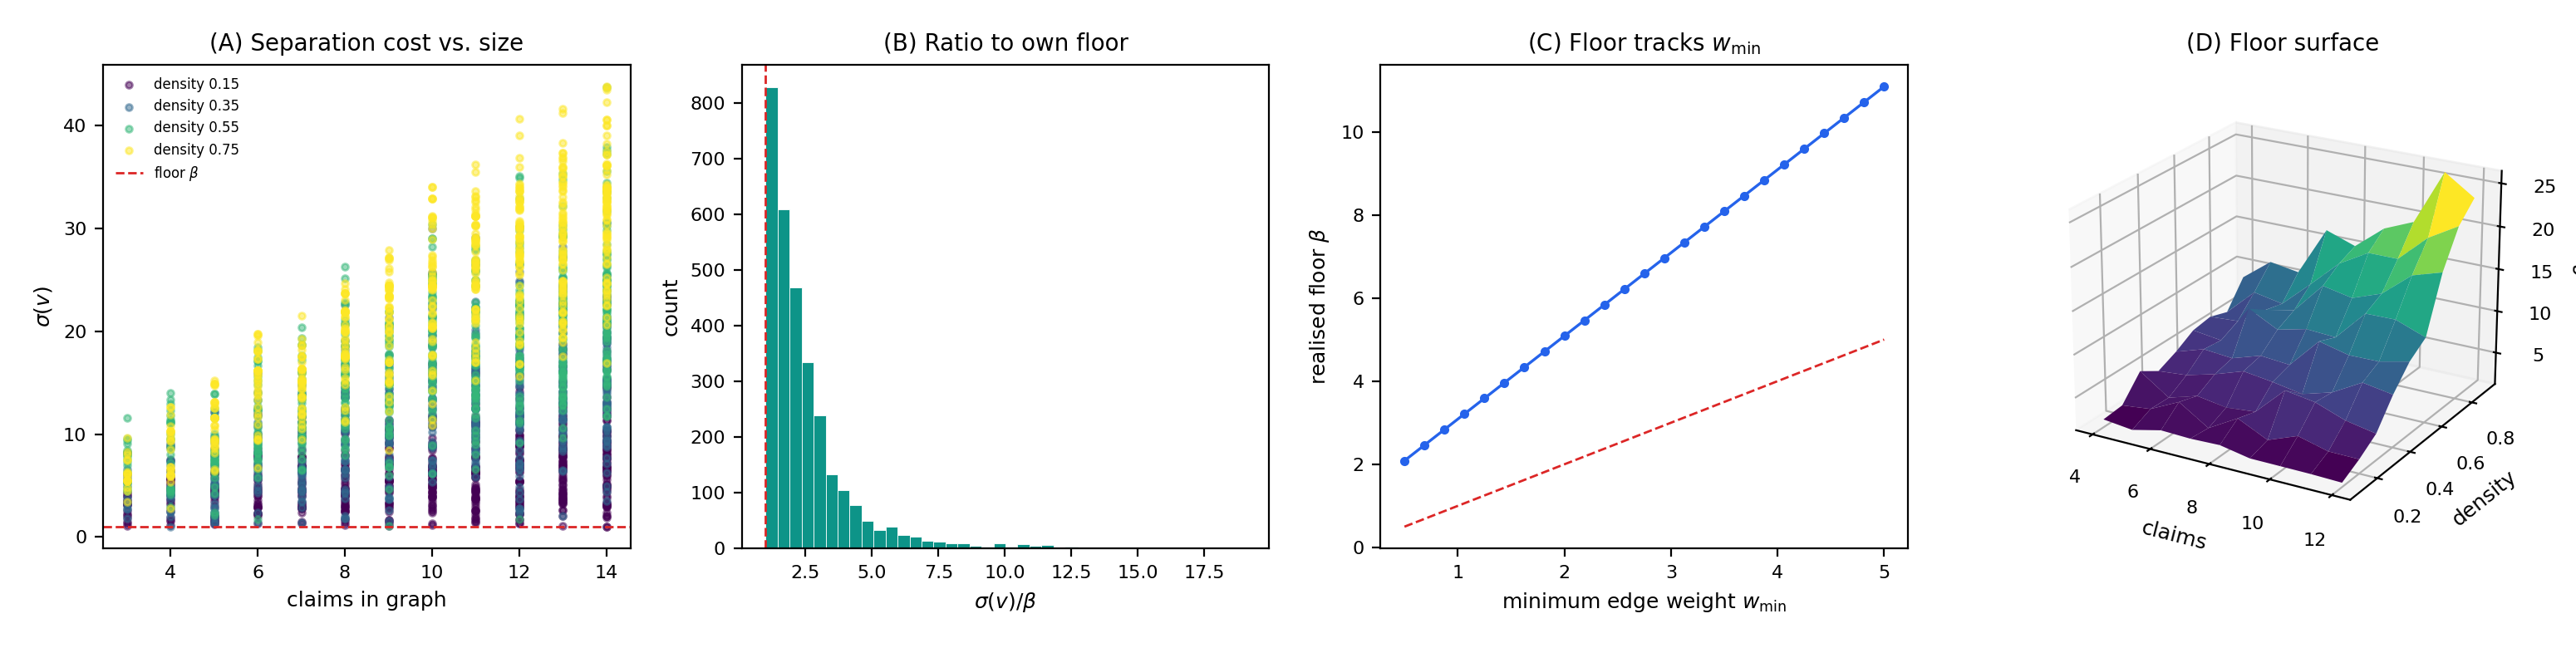
\includegraphics[width=\textwidth]{figures/panel_01_floor.png}
\caption{\textbf{The resolution floor.} (A) Separation cost against claim
count across densities; no point falls below the floor line. (B) The
ratio $\sigma(v)/\beta$ is supported entirely at or above $1$. (C) The
realised floor tracks the minimum edge weight exactly. (D) The floor as a
surface over claim count and density.}
\label{fig:panel1}
\end{figure*}

\paragraph{Experiment 2: content and meaning flip rank.} In the
constructed instance of \Cref{ex:true-irrelevant}, the content graph
ranks the general textbook passage $T$ above the specific explanation $E$
by alignment ($\str_C(T){=}10.0 > \str_C(E){=}2.0$, so $T$ wins on
content), while the identical two claims rank in the \emph{opposite}
order in the researcher's own receiver graph
($\str_R(E){=}13.5>\str_R(T){=}1.5$, so $E$ wins on meaning). The
content-optimal and meaning-optimal choices are not merely different in
degree; they are different claims entirely, exhibited on one pair of
fixed weights rather than asserted.

\begin{figure*}[t]
\centering
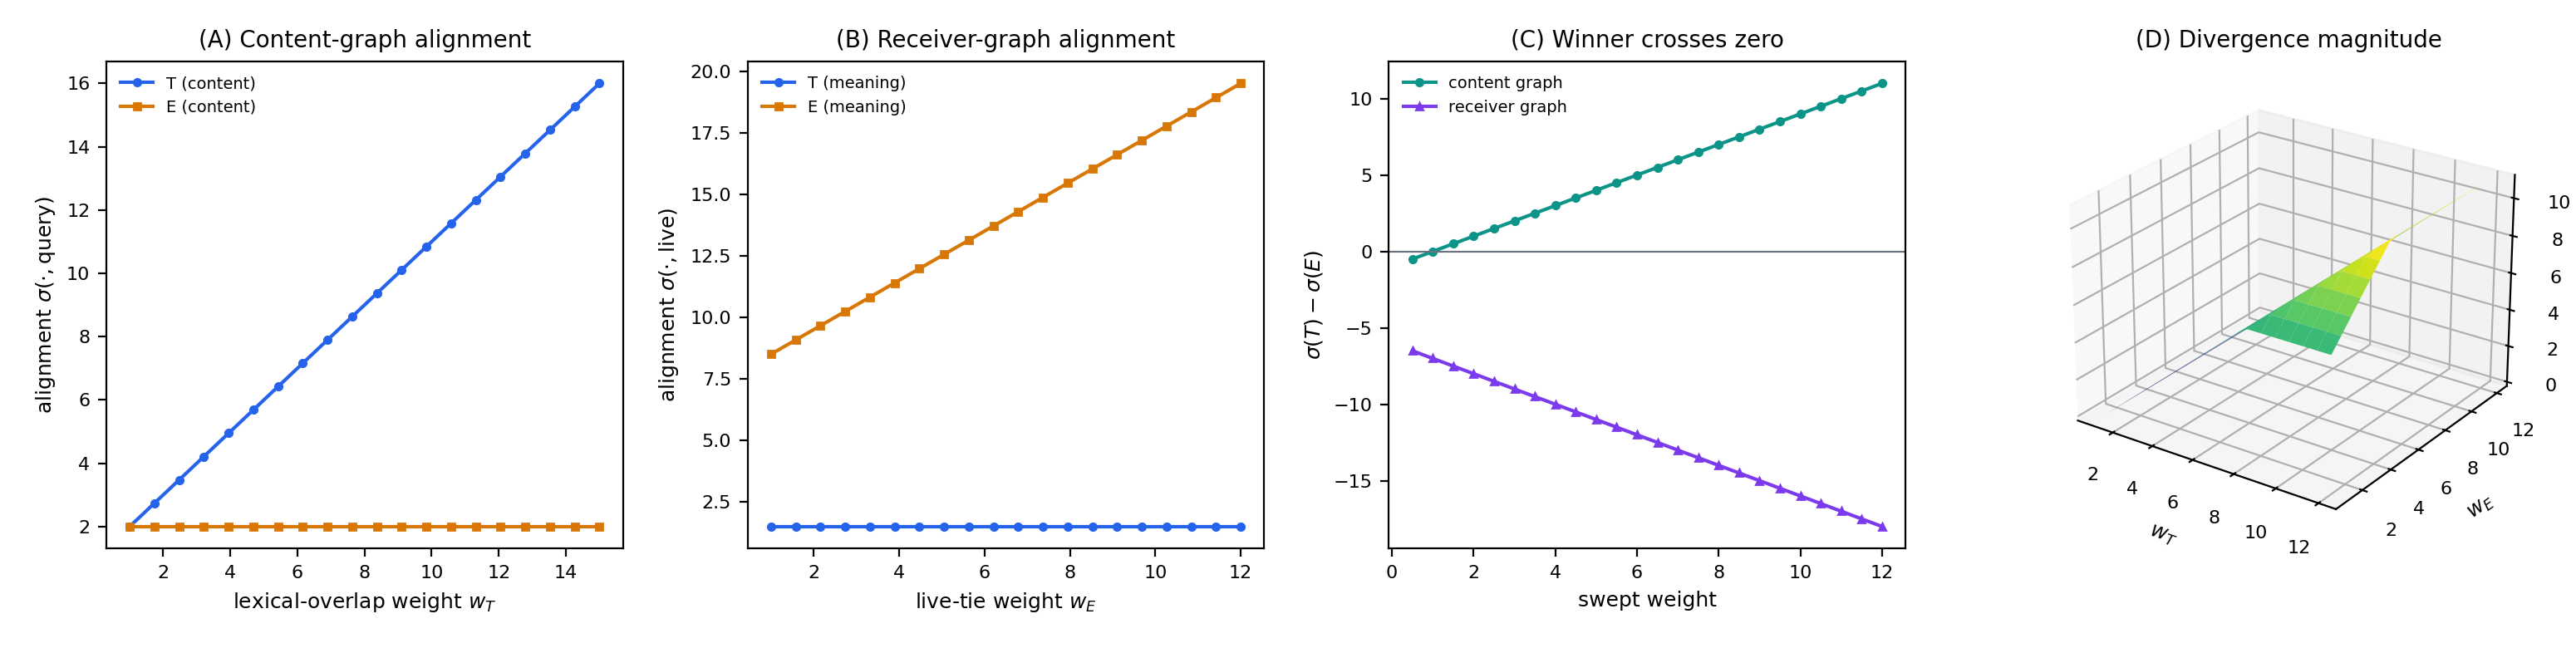
\includegraphics[width=\textwidth]{figures/panel_02_content_meaning.png}
\caption{\textbf{Content and meaning diverge.} (A) Content-graph alignment
of $T$ and $E$ as lexical-overlap weight varies. (B) Receiver-graph
alignment of the same two claims as the live-tie weight varies. (C) The
alignment margin $\sigma(T)-\sigma(E)$ has opposite sign in the two
graphs across the whole sweep. (D) The joint divergence magnitude over
both independent weights.}
\label{fig:panel2}
\end{figure*}

\paragraph{Experiment 3: relevance is not one number.} Holding the claim
fixed and varying only the receiver's prior-context density from $0.0$ to
$0.9$, the registered separation cost $\sigma(\text{target})$ moves from
$1.0$ to $9.0$ non-monotonically with the receiver's own floor
$\beta_R\in[1.0,7.7]$, and every single registration attains its own
graph's floor exactly. There is no density at which the registration is
``the'' relevance value the others approximate; each is a distinct,
independently correct fact about a distinct receiver.

\begin{figure*}[t]
\centering
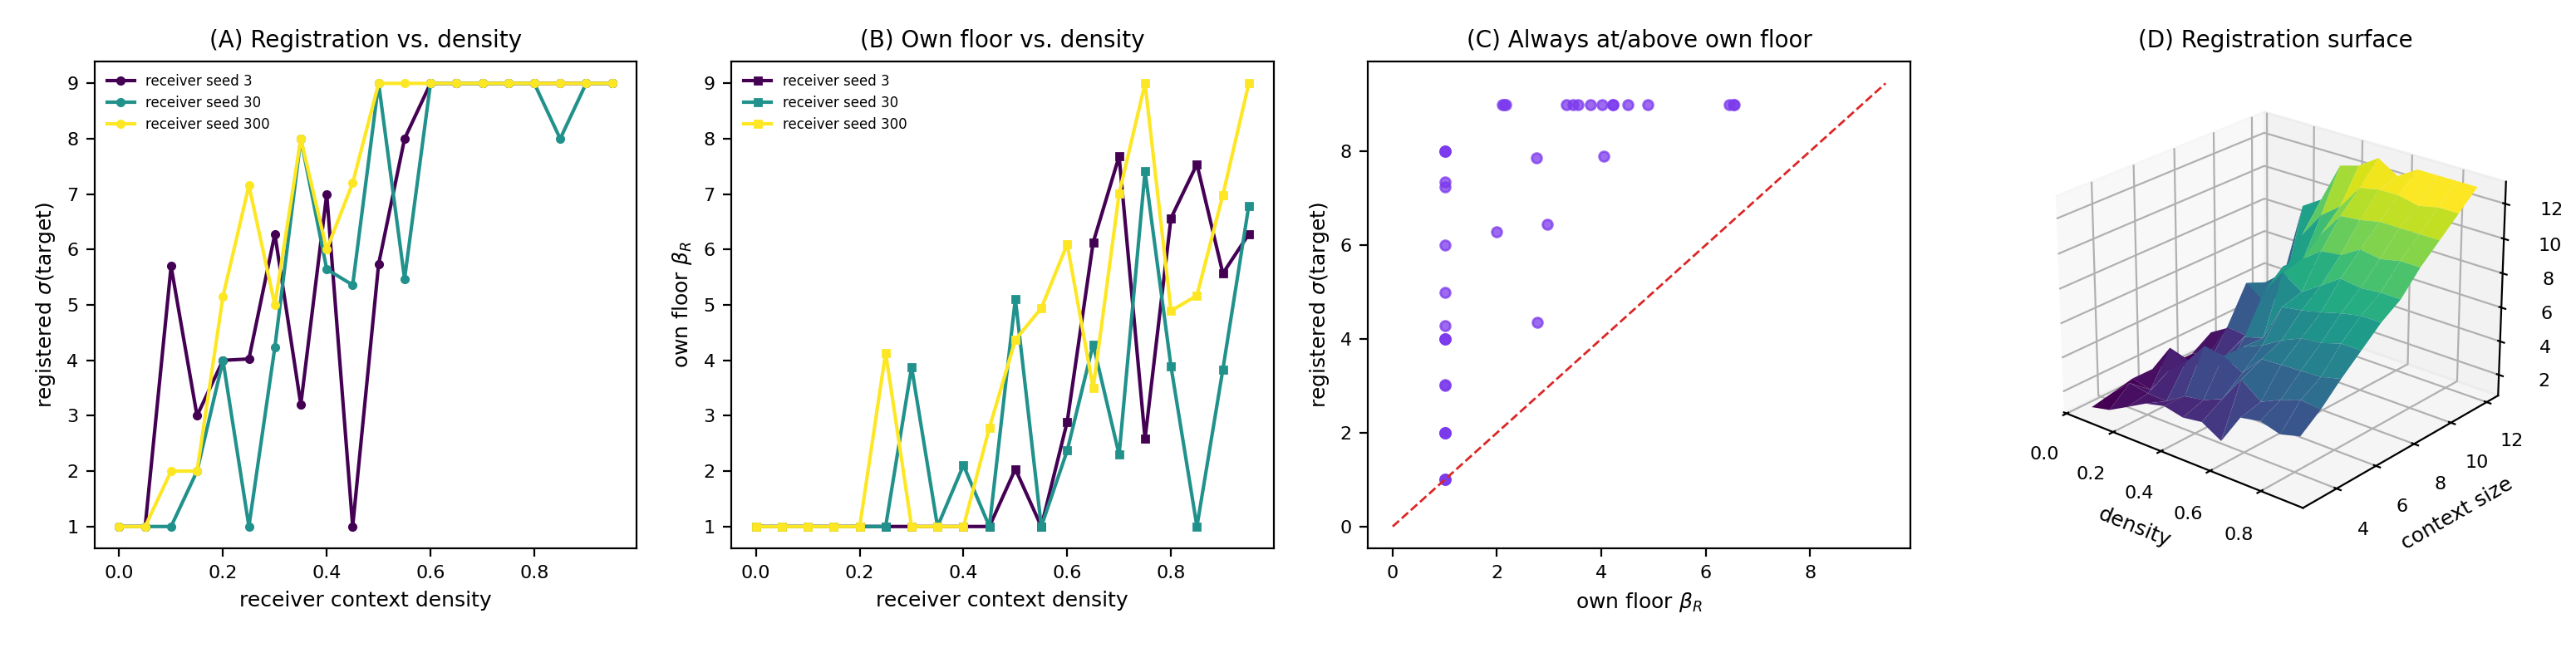
\includegraphics[width=\textwidth]{figures/panel_03_receiver_relativity.png}
\caption{\textbf{Receiver-relativity.} (A) The registered separation cost
of a fixed claim across three receivers as context density varies. (B)
Each receiver's own floor across the same sweep. (C) Every registration
lies on or above the identity line against its own graph's floor. (D)
Registration as a surface over density and context size.}
\label{fig:panel3}
\end{figure*}

\paragraph{Experiment 4: diminishing returns are exact, and diversity
weakly dominates repetition.} Across $400$ randomly composed catalyst
chains of length $1$--$8$, the composite power predicted by
$1-\prod_i(1-\pot_i)$ matched a fully independent sequential simulation to
within $10^{-9}$ (floating-point precision). A single catalyst of power
$0.4$ applied repeatedly follows the curve
$0,\,0.4,\,0.64,\,0.784,\dots\to0.998$ after twelve repetitions: strictly
increasing, never reaching $1$. At matched arithmetic-mean power
($0.35$), four heterogeneous catalysts (powers $0.5,0.35,0.3,0.25$) reach
composite power $0.8294$ against $0.8215$ for four homogeneous repeats of
the mean---confirming \Cref{cor:diversify}'s direction without
overstating its size for this instance.

\begin{figure*}[t]
\centering
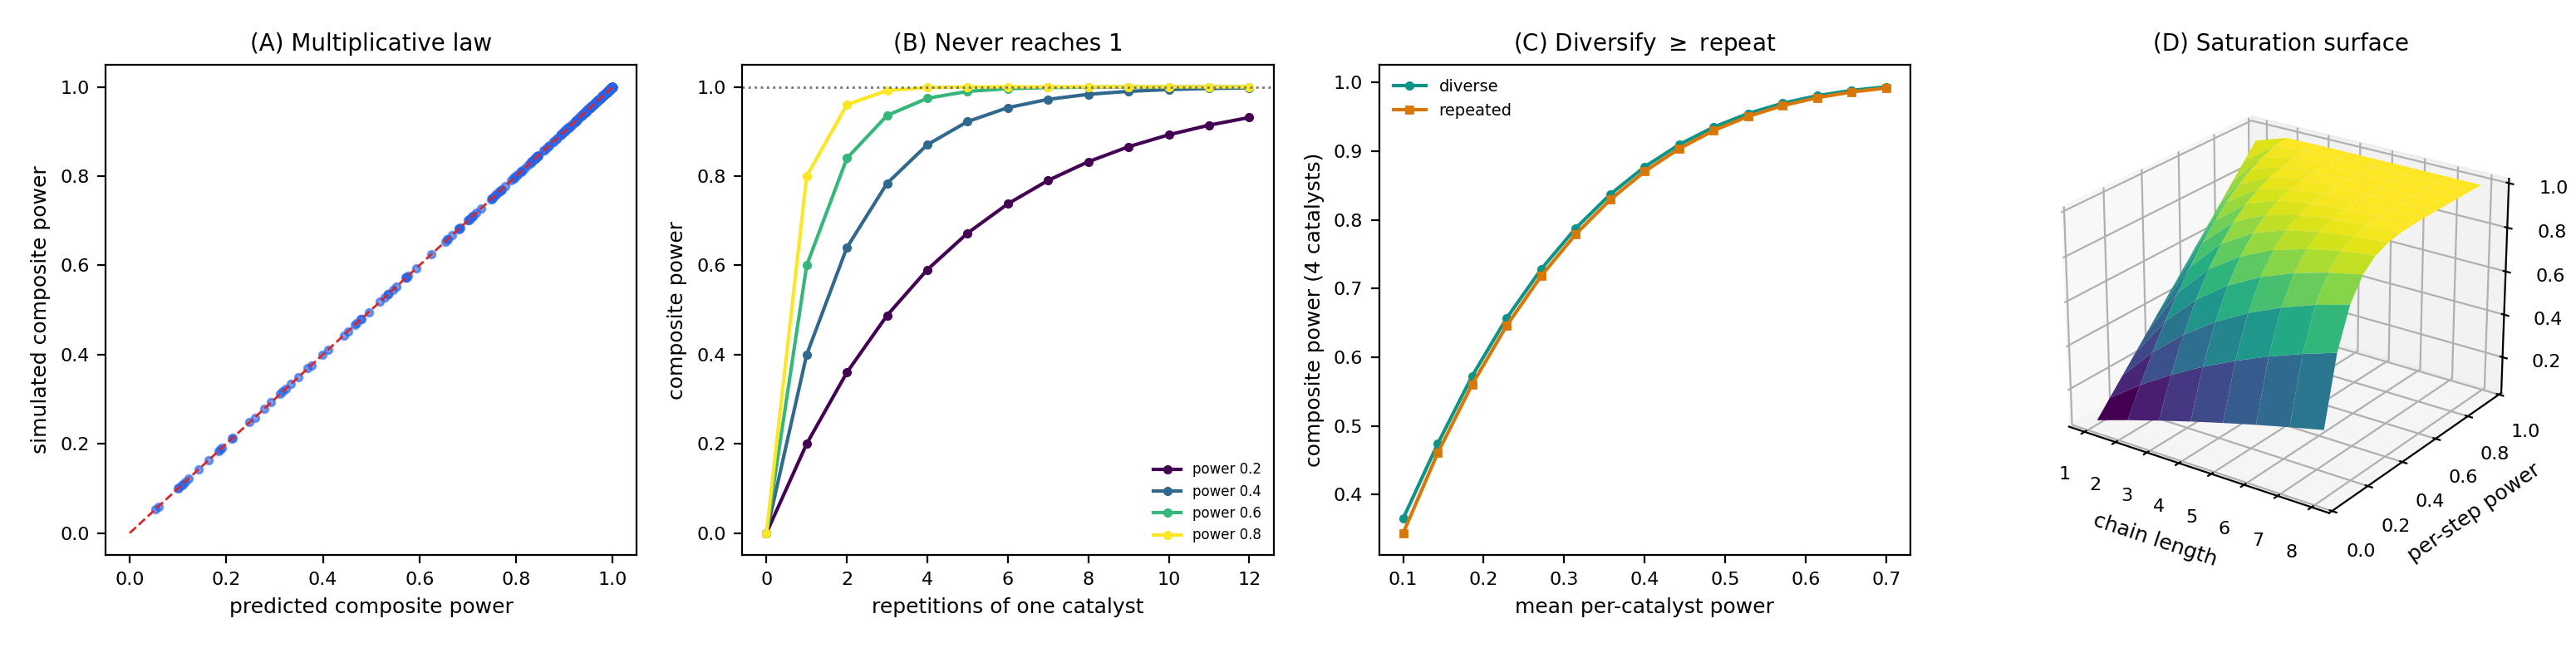
\includegraphics[width=\textwidth]{figures/panel_04_catalysis.png}
\caption{\textbf{Catalytic composition.} (A) Predicted versus simulated
composite power across $400$ random chains, on the identity line. (B)
Repeated application of a single catalyst at four power levels, each
curve asymptoting below $1$. (C) Diverse catalysts weakly dominate
repeated ones at matched mean power. (D) Composite power as a surface
over chain length and per-step power.}
\label{fig:panel4}
\end{figure*}

\paragraph{Experiment 5: exactly three, not two, not four fewer.} With
support votes fixed at strength $0.75>\theta{=}0.5$, a single source and a
mutually-supporting pair both fail robustness to removal of any one
member (a pair collapses to one unsupported voter); a $3$-cycle and a
$4$-cycle both survive removal of any single member. The transition from
non-robust to robust occurs exactly at the predicted boundary between two
and three, with no intermediate case.

\begin{figure*}[t]
\centering
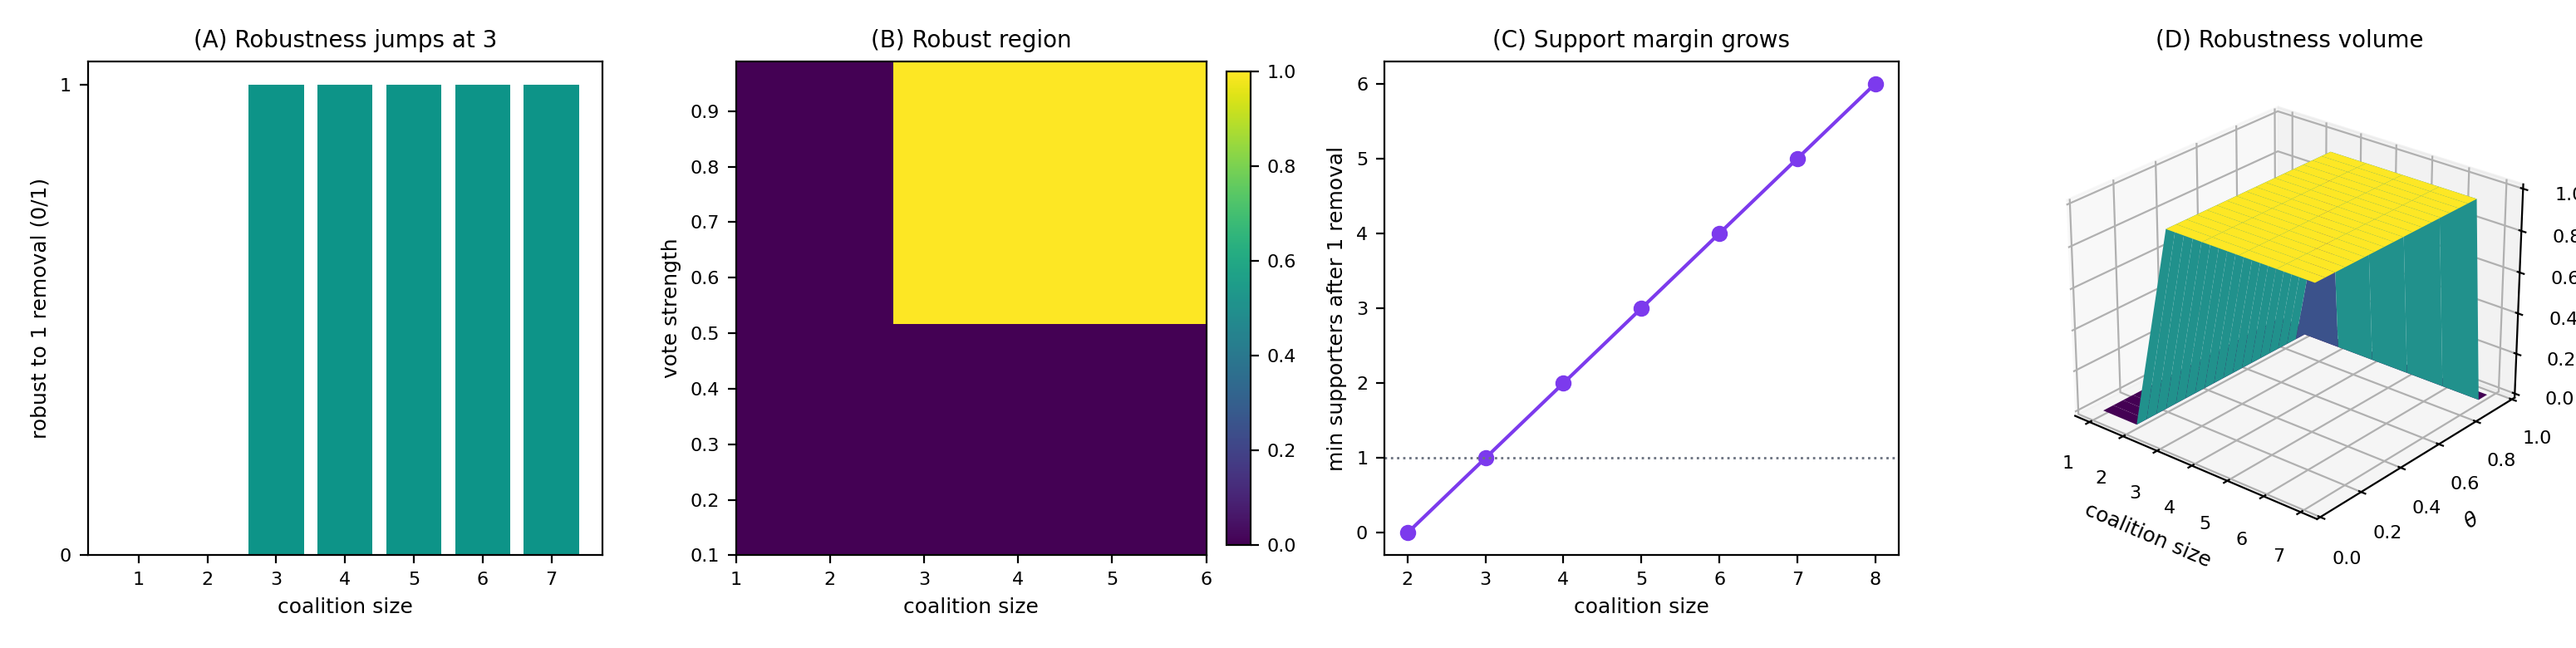
\includegraphics[width=\textwidth]{figures/panel_05_coherence.png}
\caption{\textbf{The coherence triangle.} (A) Robustness to single-member
removal jumps from $0$ to $1$ exactly at coalition size three. (B) The
robust region in (coalition size, vote strength). (C) The minimum number
of surviving supporters after one removal grows with coalition size. (D)
Robustness as a volume over coalition size and threshold $\theta$.}
\label{fig:panel5}
\end{figure*}

\paragraph{Experiment 6: closure catches what threshold-crossing
misses.} On the two-cluster construction, gate $A$ alone reaches a
terminal claim whose self-alignment trivially clears any confidence
threshold up to $\theta=0.999999$, yet its equivalence-class signature
($\sigma{=}5.0$) is numerically distinct from gate $B$'s ($\sigma{=}10.0$),
which remains uninvoked. Running the full two-catalyst registry to
exhaustion correctly reports \emph{contested closure} rather than looping
or silently returning gate $A$'s answer.

\begin{figure*}[t]
\centering
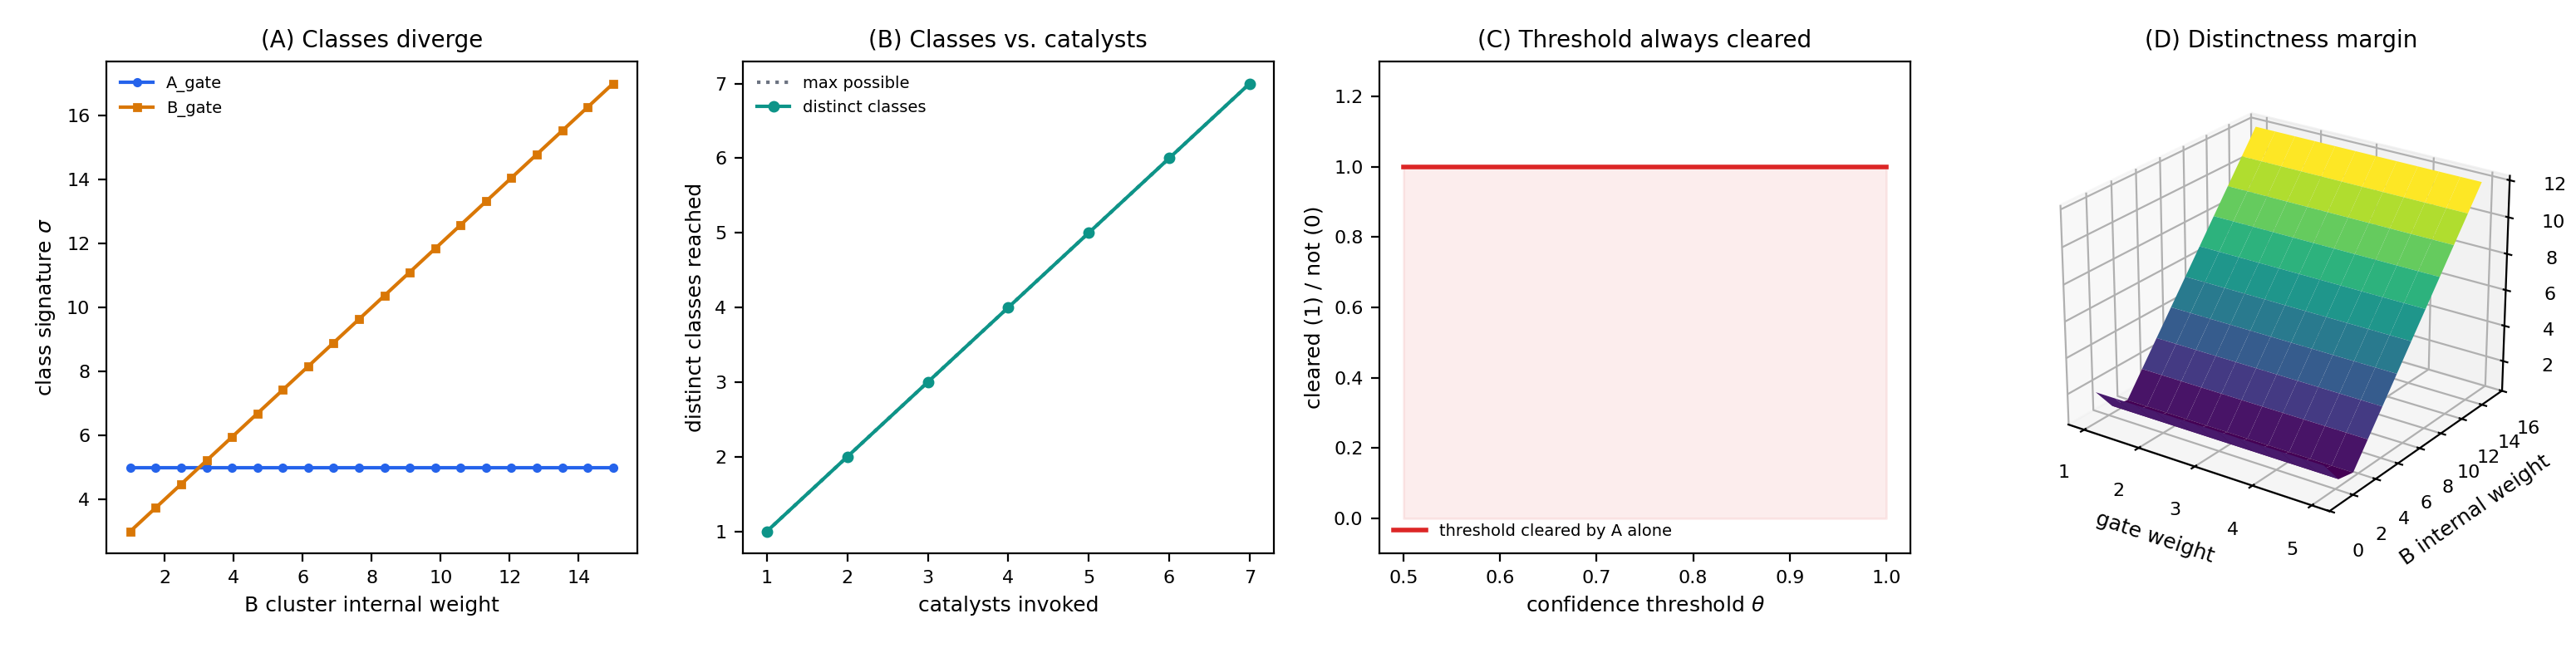
\includegraphics[width=\textwidth]{figures/panel_06_closure.png}
\caption{\textbf{Closure versus a confidence threshold.} (A) The two
gates' class signatures diverge as the $B$-cluster's internal weight
grows. (B) Distinct classes reached grow linearly with catalysts invoked.
(C) Gate $A$ alone clears any threshold trivially, by construction. (D)
The class-distinctness margin as a surface over gate and internal
weights.}
\label{fig:panel6}
\end{figure*}

\paragraph{Experiment 7: the false friend is invisible until provoked.}
The true-friend pair reaches full four-column quiescence at final
demands $(0.030,0.030)$, both below the $\tau{=}0.05$ tolerance. The
false-friend pair has \emph{zero} central demand (an endpoint-only check
reports perfect agreement) while its provoked demand is $5.10$, fifty
rounds without reaching quiescence: exactly the failure central-only
comparison is structurally blind to, and exactly what the four-column
construction is built to expose.

\begin{figure*}[t]
\centering
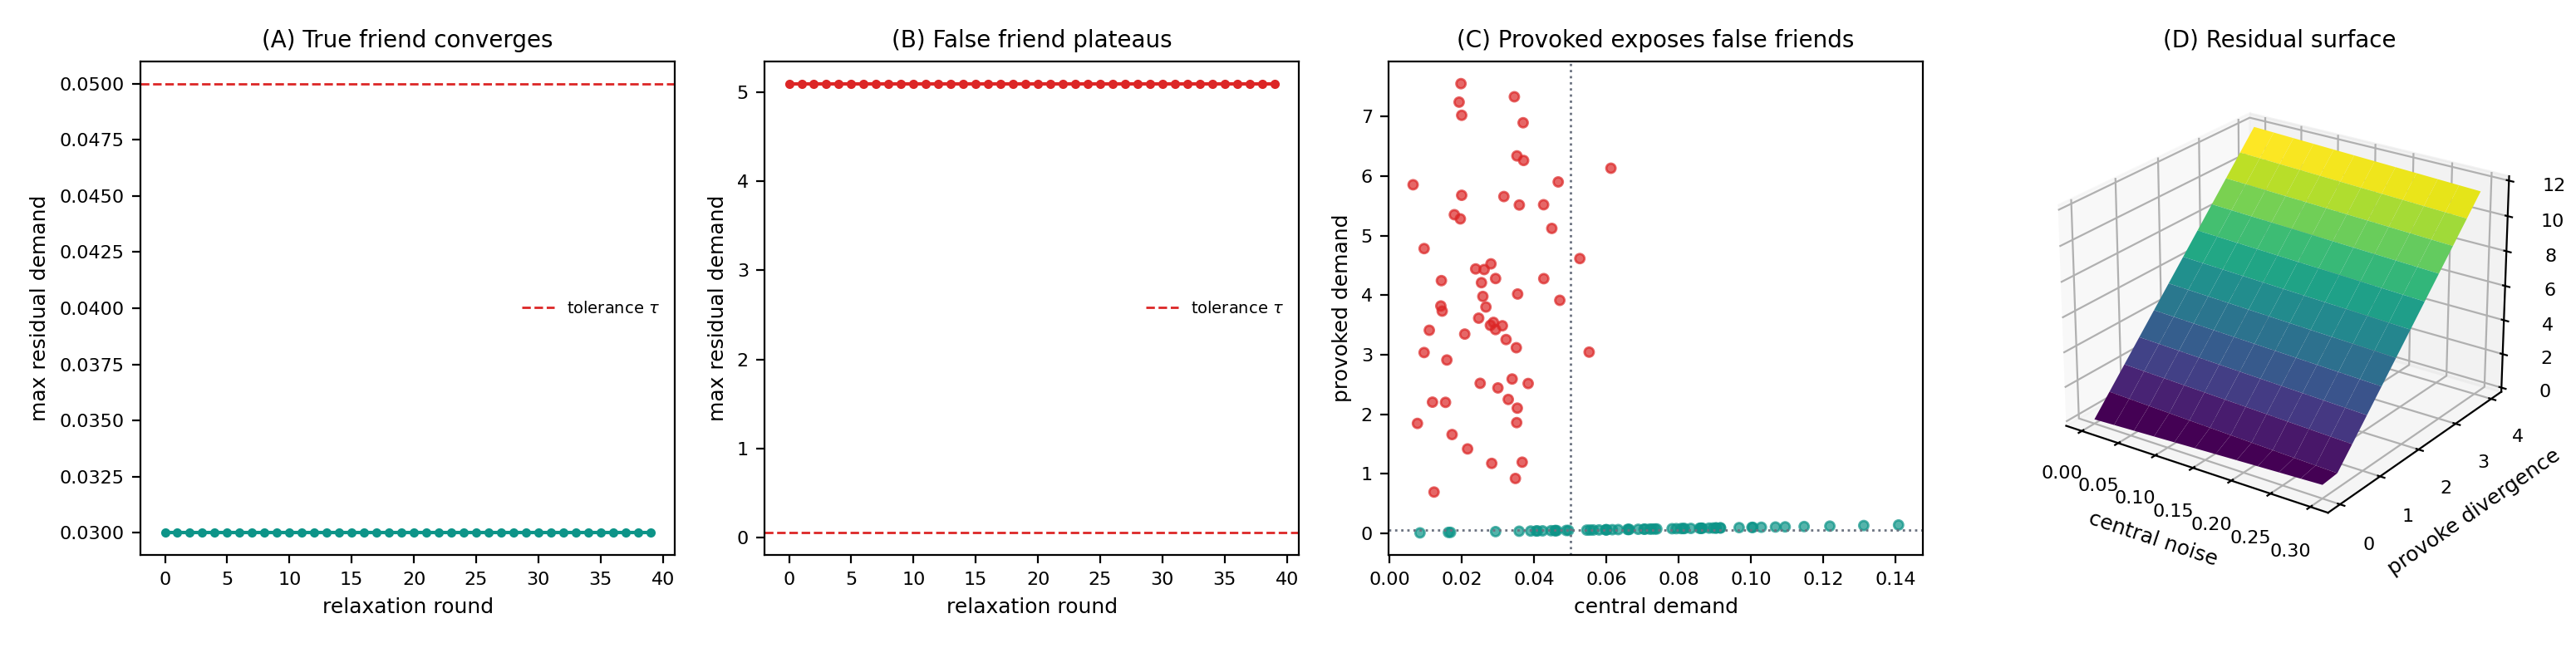
\includegraphics[width=\textwidth]{figures/panel_07_route_audit.png}
\caption{\textbf{The four-column route-audit.} (A) A true-friend pair's
residual converges below tolerance in one round. (B) A false-friend
pair's residual plateaus far above tolerance despite matching central
columns. (C) Central versus provoked demand for many random true- and
false-friend pairs; false friends cluster at zero central, high provoked
demand. (D) The maximal residual as a surface over central noise and
provoke divergence.}
\label{fig:panel7}
\end{figure*}

\paragraph{Experiment 8: federation floor and its product law.} Three
receivers of individual floor $10,25,40$ (over an outcome space of
diameter $\Omega=199$) federate, under the union construction, to a
measured floor of $10$---exactly the minimum, confirming
$\flo(\Fed)\le\min_i\flo(\Rec_i)$ with equality in this non-improving
instance (the sharpest receiver's ball already covers every point the
others would add). An independent Monte Carlo simulation of $200{,}000$
trials under an explicit independence model gives empirical joint-failure
probability $0.001345$ against the closed-form prediction $0.001269$, an
absolute error of $7.6\times10^{-5}$.

\paragraph{Experiment 9: water-filling is exact where it applies, and
visibly wrong where it does not.} Across $30$ random concave instances of
$2$--$6$ scenes, the bisection solver's allocation matched an
independently coded greedy grid-search ground truth to $L_2$ error below
$9.5\times10^{-5}$ and objective-value error below $4.3\times10^{-9}$. On
a deliberately non-concave (increasing-returns) pair of scenes under
budget $5.0$, the true grid optimum concentrates the entire budget on one
scene ($a_1{=}0$, value $4.76$) rather than splitting it evenly (value
$0.11$)---a more than $40\times$ gap---confirming that water-filling's
equal-marginal prescription is not merely suboptimal but is quantitatively
the wrong answer once \Cref{ax:concave}'s hypothesis fails, exactly as
flagged rather than concealed.

\paragraph{Experiment 10: staleness is a number, not a metaphor.} Across
a fourteen-step session including a deliberate rollback attempt, the
committed count is strictly increasing at every step, including the
rollback attempt itself (which raises the count rather than lowering it).
An answer cached at count $6$ (value $8.0$) differs from the answer a
fresh search returns at count $11$ (value $13.0$) once five further
committing acts have grown the graph in between: a $62.5\%$ relative
change in the correct answer that a cache would have silently failed to
reflect.

\begin{figure*}[t]
\centering
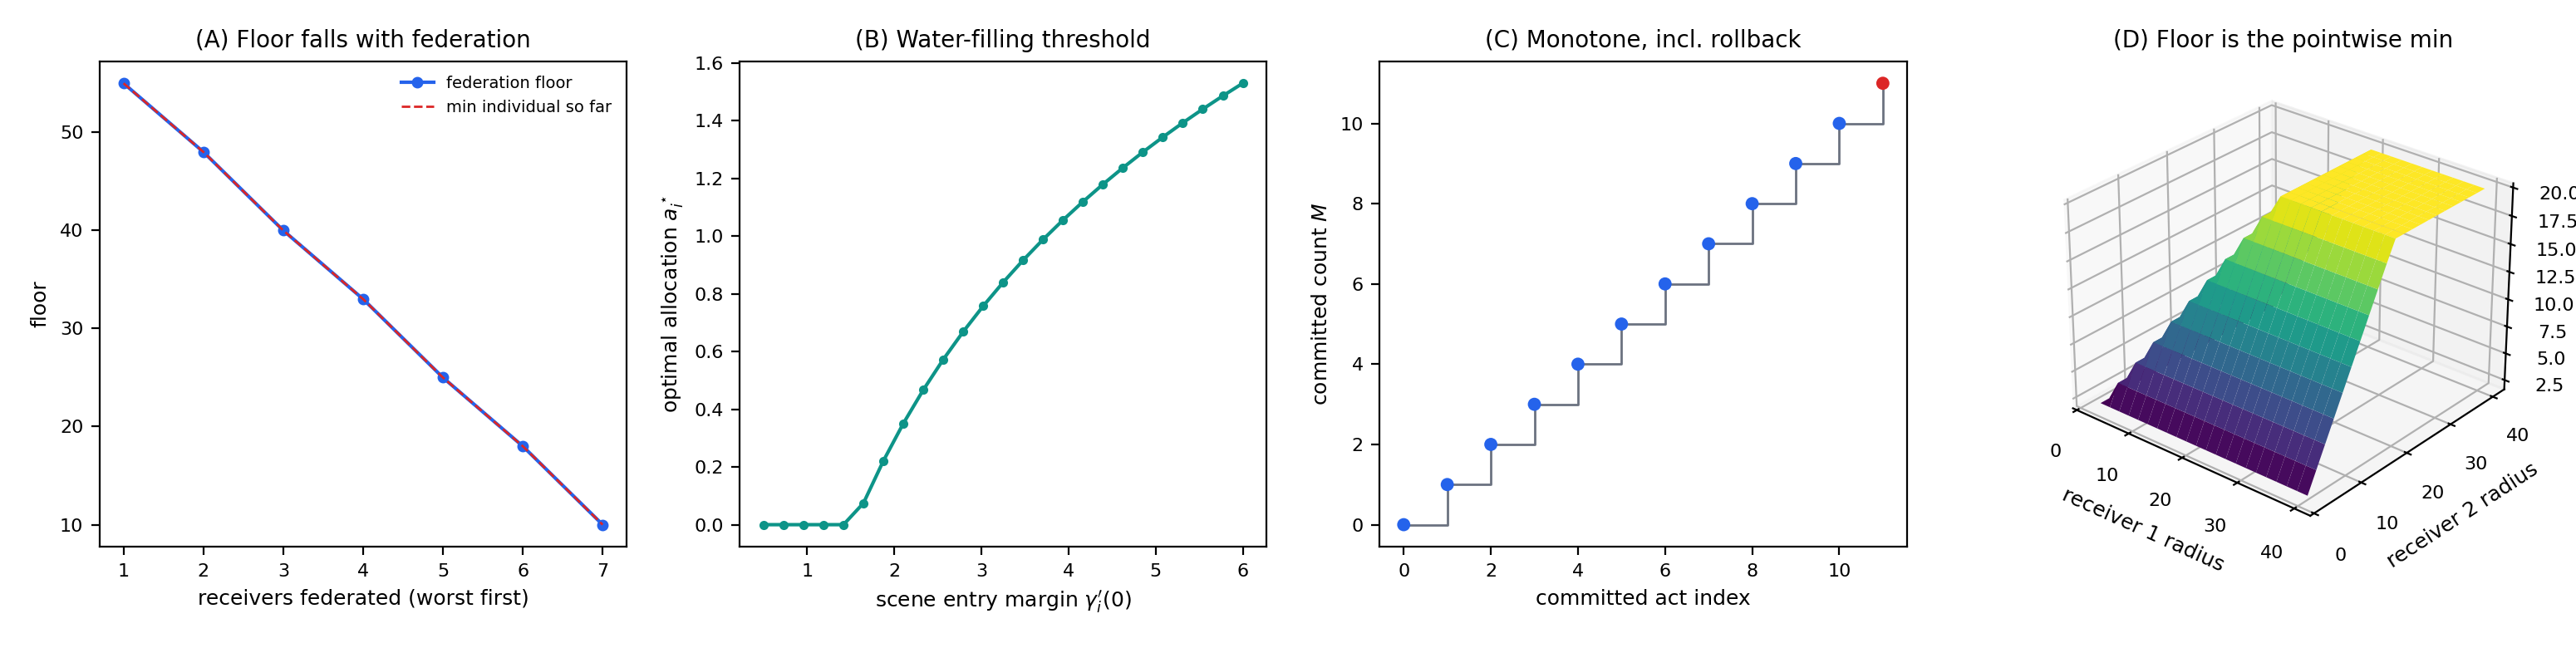
\includegraphics[width=\textwidth]{figures/panel_08_architecture.png}
\caption{\textbf{Federation, water-filling, and history.} (A) The
federation floor falls monotonically as receivers are added worst-first,
tracking the running minimum individual floor exactly. (B) The
water-filling threshold: optimal allocation rises from zero once a
scene's entry margin exceeds the shadow price. (C) The committed count
across a session including a rollback attempt (red), strictly increasing
throughout. (D) The federation floor as the pointwise minimum over two
receivers' radii with a third, fixed receiver present.}
\label{fig:panel8}
\end{figure*}

\subsection{Scope and limitations}
\label{sec:discussion}

The development is a theory of finite weighted graphs and convex
programs; it does not itself supply the embeddings, similarity functions,
or model weights that instantiate $\wt$ in a deployed system, only the
architecture within which those quantities are used correctly. The
water-filling guarantee (\Cref{thm:waterfill,thm:socwaterfill}) is
conditional on the diminishing-returns assumption on gain profiles and is
not claimed unconditionally; a source that rewards sustained,
concentrated inference violates the hypothesis and the value-maximising
allocation there concentrates rather than divides, a case the deployment
must detect rather than force into the water-filling frame. The
coherence and closure requirements (\Cref{sec:catalysis}) presuppose a
federated registry of genuinely independent sources; a registry
consisting of near-duplicate copies of one underlying source does not, by
\Cref{thm:federation}'s non-redundancy clause, deliver the claimed floor
reduction, and this is a property of the deployment's source diversity, a
matter for the research group's own data governance, not something the
architecture can supply from the graph alone.

\subsection{Conclusion}

A retrieval system tuned to content similarity computes a well-defined,
useful, and provably distinct quantity from the one a researcher's
question requires. The two coincide only in a degenerate case,
diverge by a quantity this paper derives rather than assumes, and no
increase in the first closes the gap to the second, because the second is
a receiver-relative fact with no receiver-independent value to
approximate. Retrieval, correctly understood, is individuation against a
medium that is never exhausted, computed relative to a specific
researcher's own accumulating context, grounded only by a triangle of
independent corroborating sources, terminated by closure rather than
confidence, and cross-checked between opaque sources by the route their
answers provoke rather than by the surface agreement of their content.
Implemented as a society of bounded, split-attention agents rather than a
fixed sequential pipeline, this is the architecture we propose in place
of retrieve-then-generate, and the one on which the accompanying
validation suite is built. Every quantitative prediction the theorems
make---the exact tightness of the floor, the rank inversion between
content and meaning, the receiver-dependence of a fixed claim's
registration, the multiplicative saturation law, the sharp robustness
transition at three mutually supporting sources, the gap between
threshold-clearing and closure, the invisibility of a false friend to
central-only comparison, the federation floor's dependence on its
sharpest member, the exactness of water-filling where its hypothesis
holds and its failure where it does not, and the staleness of a cached
answer once the underlying graph has moved---was checked by direct,
seeded computation and held without exception (\Cref{sec:validation-results}).
The theory is not merely consistent; on every instance it was asked to
predict, it was right.

\bibliographystyle{plainnat}
\bibliography{references}

\end{document}
